\documentclass{article}

% if you need to pass options to natbib, use, e.g.:
%     \PassOptionsToPackage{numbers, compress}{natbib}
% before loading neurips_2019

% ready for submission
% \usepackage{neurips_2019}

% to compile a preprint version, e.g., for submission to arXiv, add add the
% [preprint] option:
%     \usepackage[preprint]{neurips_2019}

% to compile a camera-ready version, add the [final] option, e.g.:
\usepackage[]{neurips_2019}

\usepackage{makecell}
\usepackage{tabularx}

% to avoid loading the natbib package, add option nonatbib:
%     \usepackage[nonatbib]{neurips_2019}

\usepackage[utf8]{inputenc} % allow utf-8 input
\usepackage[T1]{fontenc}    % use 8-bit T1 fonts
\usepackage{hyperref}% hyperlinks
\usepackage{url}            % simple URL typesetting
\usepackage{booktabs}       % professional-quality tables
\usepackage{amsfonts}       % blackboard math symbols
\usepackage{nicefrac}       % compact symbols for 1/2, etc.
\usepackage{microtype}      % microtypography
\usepackage{mwe} % For dummy images
\usepackage{subcaption}

\usepackage{bm}
\usepackage{todonotes}

\title{Re-Hamiltonian Generative Networks}

% The \author macro works with any number of authors. There are two commands
% used to separate the names and addresses of multiple authors: \And and \AND.
%
% Using \And between authors leaves it to LaTeX to determine where to break the
% lines. Using \AND forces a line break at that point. So, if LaTeX puts 3 of 4
% authors names on the first line, and the last on the second line, try using
% \AND instead of \And before the third author name.

\makeatletter
\newcommand{\printfnsymbol}[1]{%
  \textsuperscript{\@fnsymbol{#1}}%
}
\makeatother

\author{%
  Carles Balsells Rodas \thanks{Equal contribution.}\\
  KTH Royal Institute of Technology\\
  \texttt{carlesbr@kth.se}\\
   \And
   Oleguer Canal Anton \printfnsymbol{1}\\
   KTH Royal Institute of Technology \\
  % Address \\
   \texttt{oleguer@kth.se} \\
   \And
   Federico Taschin \printfnsymbol{1}\\
   KTH Royal Institute of Technology \\
  % Address \\
   \texttt{taschin@kth.se} \\
  % \And
  % Coauthor \\
  % Affiliation \\
  % Address \\
  % \texttt{email} \\
  % \And
  % Coauthor \\
  % Affiliation \\
  % Address \\
  % \texttt{email} \\
}

\begin{document}

\maketitle

\section*{\centering Reproducibility Summary}

% \textit{Template and style guide to \href{https://paperswithcode.com/rc2020}{ML Reproducibility Challenge 2020}. The following section of Reproducibility Summary is \textbf{mandatory}. This summary \textbf{must fit} in the first page, no exception will be allowed. When submitting your report in OpenReview, copy the entire summary and paste it in the abstract input field, where the sections must be separated with a blank line.
% }

\subsection*{Scope of Reproducibility}

% State the main claim of the original paper you are trying to reproduce. We recommend picking the central claim of the paper. 
The main objective of the paper is to "learn the Hamiltonian dynamics of simple physical systems from high-dimensional observations without restrictive domain assumptions".
To do so, the authors train a generative model that reconstructs an inputted sequence of images of the evolution of some physical system.
For instance, they learn the dynamics of a pendulum, a body-spring system, and 2,3-bodies.
In addition to these environments, we further expand the testing on two new environments and we explore architecture tweaks looking for performance gains.

\subsection*{Methodology}

% Briefly describe what you did and which resources did you use. E.g. Did you use author's code, did you re-implement parts of the pipeline, how much time did it take to produce the results, what hardware you were using and how long it took to train/evaluate. 
We implement the project with Python using Pytorch \cite{pytorch} as a deep learning library.
Previous to ours, there was no public implementation of this work.
Thus, we had to write the code of the simulated environments, the deep models, and the training process.
The code can be found in this repository: \href{https://github.com/CampusAI/Hamiltonian-Generative-Networks}{https://github.com/CampusAI/Hamiltonian-Generative-Networks}
A single training takes around 4 hours and 1910MB of GPU memory (NVIDIA GeForce RTX2080Ti).


\subsection*{Results}

% Start with your overall conclusion - where was your study successful and where not successful. Be specific and use precise language, e.g. "we reproduced the accuracy to within 1\% of reported value, that upholds the paper's conclusion that it performs much better than baselines". Getting exactly the same number is in most cases infeasible, so you'll need to use your judgement call to decide if your results support the original claim of the paper. 
We found the model's input-output data slightly unclear in the original paper.
First, it seems that the model reconstructs the same sequence that has been inputted.
Nevertheless, further discussion with the authors seems to indicate that they input the first few frames to the network and reconstructed the rest of the rollout.
We test both approaches and analyze the results.
We generally obtain comparable results to those of the original authors when just reconstructing the input sequence ($30\%$ average absolute relative error w.r.t. to their reported values) and worse results when trying to reconstruct unseen frames ($107\%$ error).
In this report, we include our intuition on possible reasons that would explain these observations.


\subsection*{What was easy}

% Describe which parts of your reproduction study were easy. E.g. was it easy to run the author's code, or easy to re-implement their method based on the description in the paper. The goal of this section is to summarize to the reader which parts of the original paper they could easily apply to their problem. 
The architecture of the model and training procedure was easy to understand from the paper.
Besides, creating simulation environments similar to those of the original authors was also straightforward. 

\subsection*{What was difficult}

% Describe which parts of your reproduction study were difficult or took much more time than you expected. Perhaps the data was not available and you couldn't verify some experiments, or the author's code was broken and had to be debugged first. Or, perhaps some experiments just take too much time/resources to run and you couldn't verify them. The purpose of this section is to indicate to the reader which parts of the original paper are either difficult to re-use, or require a significant amount of work and resources to verify. 
While the overall model architecture and data generation were easy to understand, we encountered the optimization to be especially tricky to perform.
In particular, finding a good balance between the reconstruction loss and KL divergence loss was challenging.
We implemented GECO \cite{geco} to dynamically adapt the Lagrange multiplier but it proved to be surprisingly brittle to its hyper-parameters, resulting in very unstable behavior.
We were unable to identify the cause of the problem and ended up training with simpler techniques such as using a fixed Lagrange multiplier as presented in \cite{beta-vae}.

\subsection*{Communication with original authors}

We exchanged around 6 emails with doubts and answers with the original authors.


\newpage

% \textit{\textbf{
% The following section formatting is \textbf{optional}, you can also define sections as you deem fit.
% }}

\section{Introduction}

% A  few  sentences  placing  the  work  in  context. Limit it to a few paragraphs at most; your report is on reproducing a piece of work, you don’t have to motivate that work.

% Problem
Consider an isolated physical system with multiple bodies interacting with each other.
Let $\bm{q} \in \mathbb{R}^n$ be the vector of their positions, and $\bm{p} \in \mathbb{R}^n$ the vector of their momenta.
The Hamiltonian formalism \cite{hamilton} states that there exists a function $\mathcal{H} : (\bm{q}, \bm{p}) \in \mathbb{R}^{n + n} \rightarrow \mathbb{R}$ representing the energy of the system which relates $\bm{q}$ and $\bm{p}$ as:
\begin{equation}
\frac{\partial \bm{q}}{\partial t} = \frac{\partial \mathcal{H}}{\partial \bm{p}}, \qquad
\frac{\partial \bm{p}}{\partial t} = -\frac{\partial \mathcal{H}}{\partial \bm{q}}
\label{eq:hamilton}
\end{equation}
% Approach
In this work $\mathcal{H}$ is modeled with an artificial neural network and property \ref{eq:hamilton} is exploited to get the temporal derivatives of both $\bm{q}$ and $\bm{p}$.
One can then use a numerical integrator (see Section \ref{sec:integrators}) to solve the ODE and infer the system evolution both forward and backward in time given some initial conditions (see Figure \ref{fig:unroll}).
These initial conditions are inferred from a natural image sequence of the system evolution (see Figure \ref{fig:initial_cond}).
The authors propose a generative approach to learn low-dimensional representations of the positions and momenta $(\bm{q}_0, \bm{p}_0)$.
This allows us to sample new initial conditions and unroll previously unseen system evolutions according to the learned Hamiltonian dynamics.



\section{Scope of reproducibility}
\label{sec:claims}

In order to verify the central claims presented in the paper we focus on the following target questions:

\begin{itemize}
    \item Does \textit{RigL} outperform existing sparse-to-sparse training techniques---such as SET (\citet{Mocanu2018SET}) and SNFS (\citet{dettmers2020sparse})---and match the accuracy of dense-to-sparse training methods such as iterative pruning (\citet{to_prune_or_not})?
    
    \item \textit{RigL} requires two additional hyperparameters to tune. We investigate the sensitivity of final performance to these hyperparameters across a variety of target sparsities (Section \ref{hyperparameter-tuning}).
    
    \item How does the choice of sparsity initialization affect the final performance for a fixed parameter count and a fixed training budget (Section \ref{effect-sparsity-distribution})?
    
    \item Does redistributing layer-wise sparsity during connection updates (\citet{dettmers2020sparse}) improve \textit{RigL}'s performance? Can the final layer-wise distribution serve as a good sparsity initialization scheme (Section \ref{effect-redistribution})? 

\end{itemize}

\section{Experiment Setup}\label{sec:replication} 
In this section we will introduce the setup of the experimental evaluation performed by the authors of the PGExplainer. While replicating their evaluation, we found that a number of steps were making assumptions that were not well documented. This includes the samples used for calculating the AUC score. In this section we will spend time on these steps. Additionally, some minor mistakes made in the original evaluation were rectified during our reproduction. These changes will also be highlighted here.

The experimental setup used by the authors of the PGExplainer follows that of the GNNExplainer \cite{ying2019gnnexplainer} with a number of extensions. To clarify, the authors' proposed method serves the purpose of explaining the classification decision of a GNN. Hence, the experiments used to evaluate the PGExplainer focus on the explanations provided by the PGExplainer for the underlying model. Specifically, the evaluation is repeated for six different datasets, and thus, for six different underlying models. The six datasets span two different classification tasks; node-classification and graph-classification. 

\subsection{Datasets \hfill \texttt{[datasets/dataset\_loaders.py]}}\label{sec:datasets}
The node classification task is performed using four synthetic datasets (a-d). All of which are first introduced in the GNNExplainer paper \cite{ying2019gnnexplainer}. The graph classification task is performed using two datasets (e-f), one synthetic and one real.

A reoccurring concept in all synthetic datasets is the so called \textit{motif}. Motifs are highly structured subgraphs---e.g. 9 nodes connected in a 2D grid. These subgraphs are then expanded by attaching them to a randomly generated graph of a different structural form---e.g. Barabasi-Albert (BA) graph \cite{Barabasi99emergenceScaling} or trees. Motifs play a crucial role in determining ground-truth explanations for our evaluations, as we will see later.
% All six datasets are specified and visualised in Table \ref{tab:results} (Appendix \ref{appendix:A}) \cite{luo2020parameterized}.

(a) The BA-Shapes dataset consists of single base BA-graph with 300 nodes, 80 “house”-structured motifs---each attached to random BA nodes---and some extra randomly added edges. (b) BA-Community closely resembles BA-Shapes, connecting two BA-Shapes and utilizing a Gaussian distributions for each BA-Shape to sample node features. (c) Tree-Cycles adopts an $8$-level balanced binary tree as the base graph with a set of $80$ six-node cycle motifs attached to randomly selected nodes. (d) The Tree-Grids dataset is similar to Tree-Cycles, replacing cycle motifs with $3\times 3$ grid motifs. (e) The authors constructed the BA-2motifs dataset consisting of $1000$ BA graphs. Half of the graphs contain "house" motifs, the other half contain five-node cycle motifs attached to the BA graph. These two types of graphs serve as the two classes for the dataset. (f) The real-life Mutagenicity dataset copied from \cite{ying2019gnnexplainer}, consisting of $4337$ molecule graphs. These should be classified as either mutagenic or nonmutagenic.
% All base nodes are labelled $0$, the nodes constructing the "house"'s top, middle and bottom are labelled $1$, $2$ and $3$ respectively. 
% In BA-Community nodes are labeled based on their structural roles and community memberships, leading to $8$ classes in total.


% \begin{enumerate}[(a)]
%     \item The BA-Shapes dataset consists of single base Barabasi-Albert (BA) graph \cite{Barabasi99emergenceScaling} with 300 nodes, 80 “house”-structured motifs---each attached to random BA nodes---and some extra randomly added edges. All base nodes are labelled $0$, the nodes constructing the "house"'s top, middle and bottom are labelled $1$, $2$ and $3$ respectively. 
%     \item BA-Community closely resembles BA-Shapes, connecting two BA-Shapes and utilizing a Gaussian distributions for each BA-Shape to sample node features. In BA-Community nodes are labeled based on their structural roles and community memberships, leading to $8$ classes in total.
%     \item Tree-Cycles adopts an $8$-level balanced binary tree as the base graph with a set of $80$ six-node cycle motifs attached to randomly selected nodes.
%     \item The Tree-Grids dataset is similar to Tree-Cycles, replacing cycle motifs with $3\times 3$ grid motifs.
%     \item The authors constructed the BA-2motifs dataset consisting of $1000$ BA graphs. Half of the graphs contain "house" motifs, the other half contain five-node cycle motifs attached to the BA graph. These two types of graphs serve as the two classes for the dataset.
%     \item The real-life Mutagenicity dataset copied from         \cite{ying2019gnnexplainer}, consisting of $4337$ molecule graphs. These should be classified as either mutagenic or nonmutagenic.
% \end{enumerate}


% In order to compare and evaluate results, the authors use the four datasets found in \cite{ying2019gnnexplainer}; BA-Shapes (1), BA-Community (2), Tree-Cycles (3), and Tree-Grids (4). Additionally, they construct a fifth graph classification dataset, BA-2motifs (5). All five datasets are also specified and visualised in Table \ref{tab:dataset_info} and Table \ref{tab:results} \cite{luo2020parameterized}.
% (1) The BA-Shapes dataset consists of single base Barabasi-Albert (BA) graph \cite{Barabasi99emergenceScaling} with 300 nodes, 80 “house”-structured motifs---each attached to random BA nodes---and some extra randomly added edges. All base nodes are labelled $0$, the nodes constructing the "house"'s top, middle and bottom are labelled $1$, $2$ and $3$ respectively. 
% (2) BA-Community closely resembles BA-Shapes, connecting two BA-Shapes and utilizing a Gaussian distributions for each BA-Shape to sample node features. In BA-Community nodes are labeled based on their structural roles and community memberships, leading to $8$ classes in total.
% (3) Tree-Cycles adopts an $8$-level balanced binary tree as the base graph with a set of $80$ six-node cycle motifs attached to randomly selected nodes.
% (4) The Tree-Grids dataset is similar to Tree-Cycles, replacing cycle motifs with $3\times 3$ grid motifs.
% (5) The authors constructed the BA-2motifs dataset consisting of $1000$ BA graphs. Half of the graphs contain "house" motifs, the other half contain five-node cycle motifs attached to the BA graph. These two types of graphs serve as the two classes for the dataset.
% (6) Finally, they include the real-life MUTAG dataset copied from \cite{ying2019gnnexplainer}, consisting of $4337$ molecule graphs. These should be classified as either mutagenic or nonmutagenic.


% \begin{table}[h]
%     \centering
%     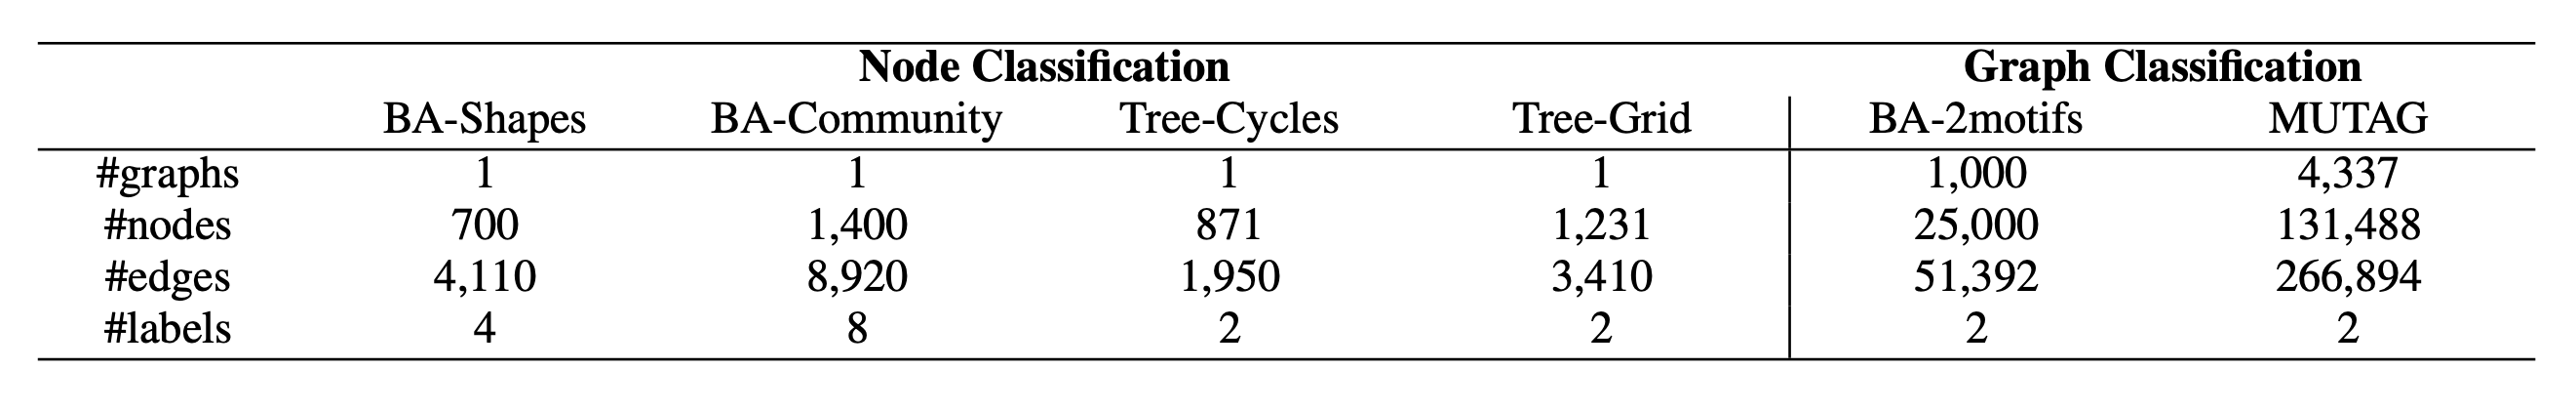
\includegraphics[width=1\linewidth]{imgs/dataset_info.png}
%     \caption{Original paper's dataset statistics \cite{luo2020parameterized}}
%     \label{tab:dataset_info}
% \end{table}

\subsection{Model \hfill \texttt{[models/GNN\_paper.py]}}
There are a number of large differences between the implementation of the models trained for each dataset and how they are described in the paper. These changes are different between the node and graph classification tasks. 

\paragraph{Node classification}
The authors describe the model for node classification to be three consecutive Graph Convolution layers feeding directly into the fully connected classification. The model in the codebase however first concatenates the three intermediate outputs of the Graph Convolution layers before using this enlarged embedding as the input for the fully connected classification layer. The coded version of the models is similar to what is used for evaluation in the GNNExplainer paper \cite{ying2019gnnexplainer}. To keep the evaluation consistent, we will therefore use the coded model version instead of the one described in the paper for our evaluation. Moreover, we were not able to get the model described in the paper to train to the same accuracy using the provided hyperparameters. 

In addition to the architecture change, we found the node classification models to use an undocumented batch normalization layer after the first and second Graph Convolution layer. Unfortunately, the original codebase contained an error that resulted in these batch-normalization layers being kept in training mode during evaluation. This observation was confirmed by the authors in communication and has since been resolved. In the same communication the authors expressed that to be able to reproduce their results, the batch normalization layers will have to be kept in training mode. We believe that this will compromise the usability of our reproducibility experiment and therefore decided to remove the batch normalization layers all together. For completeness full replication of the authors evaluation with a model containing batch normalization is included in Appendix \ref{appendix:batch_norm}.

\paragraph{Graph classification}
The graph classification models are more in line with the models described in the paper than the node classification models. The difference is the use of both max and mean pooling over the output of the final Graph Convolution layer. These two pooling types are concatenated to form inputs for fully connected layers.  

% In contrast to what is described in the paper, the model for which the PGExplainer provides explanations is considerably different from the model used in the GNNExplainer paper. Most notably, the authors included additional batch normalization layers for the first and second Graph Convolution layer. In addition to this, the implemented model does also not follow the general model structure as defined in the paper. Instead of using consecutive 3 Graph convolution layers feeding directly into the fully connected classification layer, the coded model first concatenates the three outputs of the GC layers before feeding it. 

% - Describe the model that they implemented in their code
%     - same as GNNExplainer, with additional batch normalization
% - In contrast to what is defined in the paper, the layers are concatenated
% - Use of both max and mean pooling in code, but not paper
% \paragraph{Training}
%     - As described in paper
%     - Main difference in code is longer training of the Graph classification models

\subsection{Evaluation metrics \hfill \texttt{[tasks/replication.py]}}

For each dataset, the explanations are evaluated using three broad categories; quantitative, qualitative and efficiency.

\subsubsection{Quantitative evaluation \hfill \texttt{[evaluation/AUCEvaluation.py]}}
For each dataset the explanations provided by the PGExplainer are compared to ground-truth explanations. These ground-truths describe for each sample which edges should or should not be included in the explanation. Using this methodology, the quantitative evaluation can be performed similar to a binary classification task. For this reason, the authors present the quantitative score using the AUC scoring metric. 

\paragraph{Ground Truth }
For node classification the ground-truth explanation is determined globally---i.e. for all node samples the edges have the same ground-truth explanation label. Specifically, for each edge it is determined if the two nodes it connects are part of a motif. When this is the case, the edge is labelled as positive for the ground-truth explanation. Otherwise, the edge is labelled as negative for the ground-truth explanation. For graph classifications this is dependent on the dataset used and how the ground-truth explanations are generated. For the BA-2motif dataset, being synthetic, this is done the same way as for the node datasets. The only difference being that the process is repeated for every graph in the dataset. As there are no motifs defined for the Mutagenicity dataset, the ground-truth labels can not be defined based on them. Instead, for this dataset edge labels are used, as provided by the original dataset repository\footnote{https://ls11-www.cs.tu-dortmund.de/staff/morris/graphkerneldatasets}. 

\paragraph{AUC score}
With the explanation mask provided by the PGExplainer and the ground-truths defined as above, the AUC score can be computed. However, there are a few important notes to consider when computing the AUC score. First, for the node classification datasets, the explanation mask is only determined for a 3-hop graph around each node. This is done because the GCN model only contains three layers. Second, only the nodes that are part of a motif are used in the AUC computation. This is because there is no real definition of ground-truth for the nodes outside the motifs. This evaluation design choice is further discussed in Sec.\,\ref{sec6}. Third, for the BA-2Motif dataset only a subset of the graphs is used to determine the AUC score, this is done to reduce computation time. Lastly, for the Mutagenicity dataset only the mutagenic graphs have a valid ground-truth interpretation. Hence, the AUC is determine using only these graphs. Of these four considerations, only the last is mentioned in the original paper. 

\paragraph{Comparison} The authors compare their method against four baselines; a gradient-based model (GRAD) \cite{ying2019gnnexplainer}, a graph attention network (ATT) \cite{velivckovic2017graph} and Gradient \cite{pope2019explainability}. With the exception of the scores presented for the graph-classification datasets, the scores presented are reused from the PGExplainer paper (see Table \ref{tab:results}). In communication with the authors, it was mentioned that the reimplementation of these explainers by the authors had resulted in lackluster results. For this reason the decision was made to use the original scores by the original authors. 

For our replication of the evaluation we focus our comparison on the GNNExplainer. This method is the most similar and was a major inspiration for the PGExplainer. In contrast the the original evaluation, we do perform the comparison using our own re-implementation of the GNNExplainer. Our re-implementation of this method is largely inspired by the implementation in the PyTorch Geometric library. The main difference is that our re-implementation is adapted to also work with graph-classification datasets. This is not possible with the plain PyTorch Geometric implementation. 

\subsubsection{Qualitative evaluation \hfill \texttt{[utils/plotting.py]}}
In order to obtain a visualisation of the chosen sub-graph the system takes as input the ground truth labels and the mask provided by the Explainer. Given the mask, two thresholds are calculated, one for importance to the explanation and one to determine which other elements to plot for the sub-graph. Then, using these thresholds all nodes that have an interesting enough weight are selected. Following this, only nodes that are in a direct sub-graph together the node-to-be-explained are selected. When drawing the explanation for the graph classification this sub-graph is selected using the top-$k$ edges. The original evaluation sets $k$ to be the number of edges in the defining motif for the synthetic datasets. These edges are plotted with a colour coding in accordance to their weight, where darker edges have higher weights in the mask than the lighter edges. Finally, the nodes that are connected to the previously plotted edges are plotted and colour coded by their ground-truth label.

\subsubsection{Efficiency evaluation \hfill \texttt{[evaluation/EfficiencyEvaluation.py]}}
In the paper, the authors only compare the efficiency of their PGExplainer to the GNNExplainer. Unfortunately, we were unable to extract the exact method for doing so from both the paper and the provided codebase. Our implementation is therefore mainly our own design.

We compute the inference time as the average over ten runs. During each run we measure the times it takes to explain all samples that are also used for the quantitative evaluation. This time is divided by the number of samples explained to get the final inference time per sample in milliseconds. Note that, similar to the paper, for the evaluation of the PGExplainer only the time to explain each sample is considered. On the other hand, for the GNNExplainer the time required to train the explainer is also taken into account because it has to be retrained for each sample. 

% The experimental settings closely follow those of the GNNExplainer \cite{ying2019gnnexplainer}. A three-layered GNN for each dataset is trained prior to explaining the predictions made by the GNN. 
% - Evaluation done on three levels, Qualitative, Quantitative and Inference
% - Using 2 different tasks, four datasets node classficiation and 2 datasets grap classification
% - Complete evaluation done using a single model
% \paragraph{Qualitative evaluation}
% - Single example presented for each dataset
% - Based on code the example is handpicked 
% \paragraph{Quantitative evaluation}
% - For each dataset a ground truth explanation is constructed
% - Ground truth describes for each edge if it should be included in th explanation or not. Based on this, the accuracy of the explanation can be calculated
% - Note that there are some important things to keep in mind for this way of evaluating
%     - for each dataset, a save set of nodes to perform the evaluation on is defined
%     - in case of node-classification, this is only the 3hop subgraph
%     - in case of graph-classification, this is the entire graph
% \paragraph{Efficiency evaluation}
% - Compare GNNExplainer vs. PGExplainer. Do not take into account training time for PGExplainer.
% - Different frameworks are used for both models and a different implementation style
% - No code included in the repo to reproduce this result. 

        

    
% \subsection{Results}
% \paragraph{Model training}
% In Tab.~\ref{tab:accuracies} the final accuracies of all models are provided. Note that these are the accuracies of the models that will be explained by the PGExplainer, not the explanation accuracies for the PGExplainer itself. For most models, using the configurations found in the code, we achieve results comparable to the results presented in the paper, except for the BA-Community and Mutagenicity models. 

% \begin{table}[]
% \centering
% \begin{tabular}{cccccccc}
% \toprule
% &\multicolumn{4}{c}{\textbf{Node Classification}} & \multicolumn{2}{c}{\textbf{Graph Classification}} \\
% Accuracy & \multicolumn{1}{c}{BA-Shapes} & \multicolumn{1}{c}{BA-Community} & \multicolumn{1}{c}{Tree-Cycles} & \multicolumn{1}{c|}{Tree-Grid} & \multicolumn{1}{c}{BA-2motifs} & \multicolumn{1}{c}{Mutagenicity} \\ 
% \midrule
% Training & 0.98 & 0.94 & 0.96 & \multicolumn{1}{c|}{0.96} & x.xx & 0.82 \\
% Validation & 0.99 & 0.74 & 0.99 & \multicolumn{1}{c|}{0.98} & x.xx & 0.82 \\
% Testing & 1.00 & 0.71 & 0.97 & \multicolumn{1}{c|}{0.99} & x.xx & 0.81 \\
% \bottomrule
% \end{tabular}
% \caption{Accuracies for models}
% \label{tab:accuracies}
% \end{table}

% %                 Node classification                         Graph classification
% %               Syn1, syn2m= .....                      Ba2, mutag
% % -----
% %visualization
% %------
% % PG them auc
% % PG us auc
% % ----
% % inference time
% \begin{table}[]
% \centering
% \begin{tabular}{lllllll}
% \toprule
% \multicolumn{5}{c}{\textbf{Node Classification}} & \multicolumn{2}{c}{\textbf{Graph Classification}} \\
% \multicolumn{1}{c}{} & \multicolumn{1}{c}{BA-Shapes} & \multicolumn{1}{c}{BA-Community} & \multicolumn{1}{c}{Tree-Cycles} & \multicolumn{1}{c|}{Tree-Grid} & \multicolumn{1}{c}{BA-2motifs} & \multicolumn{1}{c}{Mutagenicity} \\ \hline
% \multicolumn{7}{l}{\textbf{Visualization}} \\ \hline
% Original &  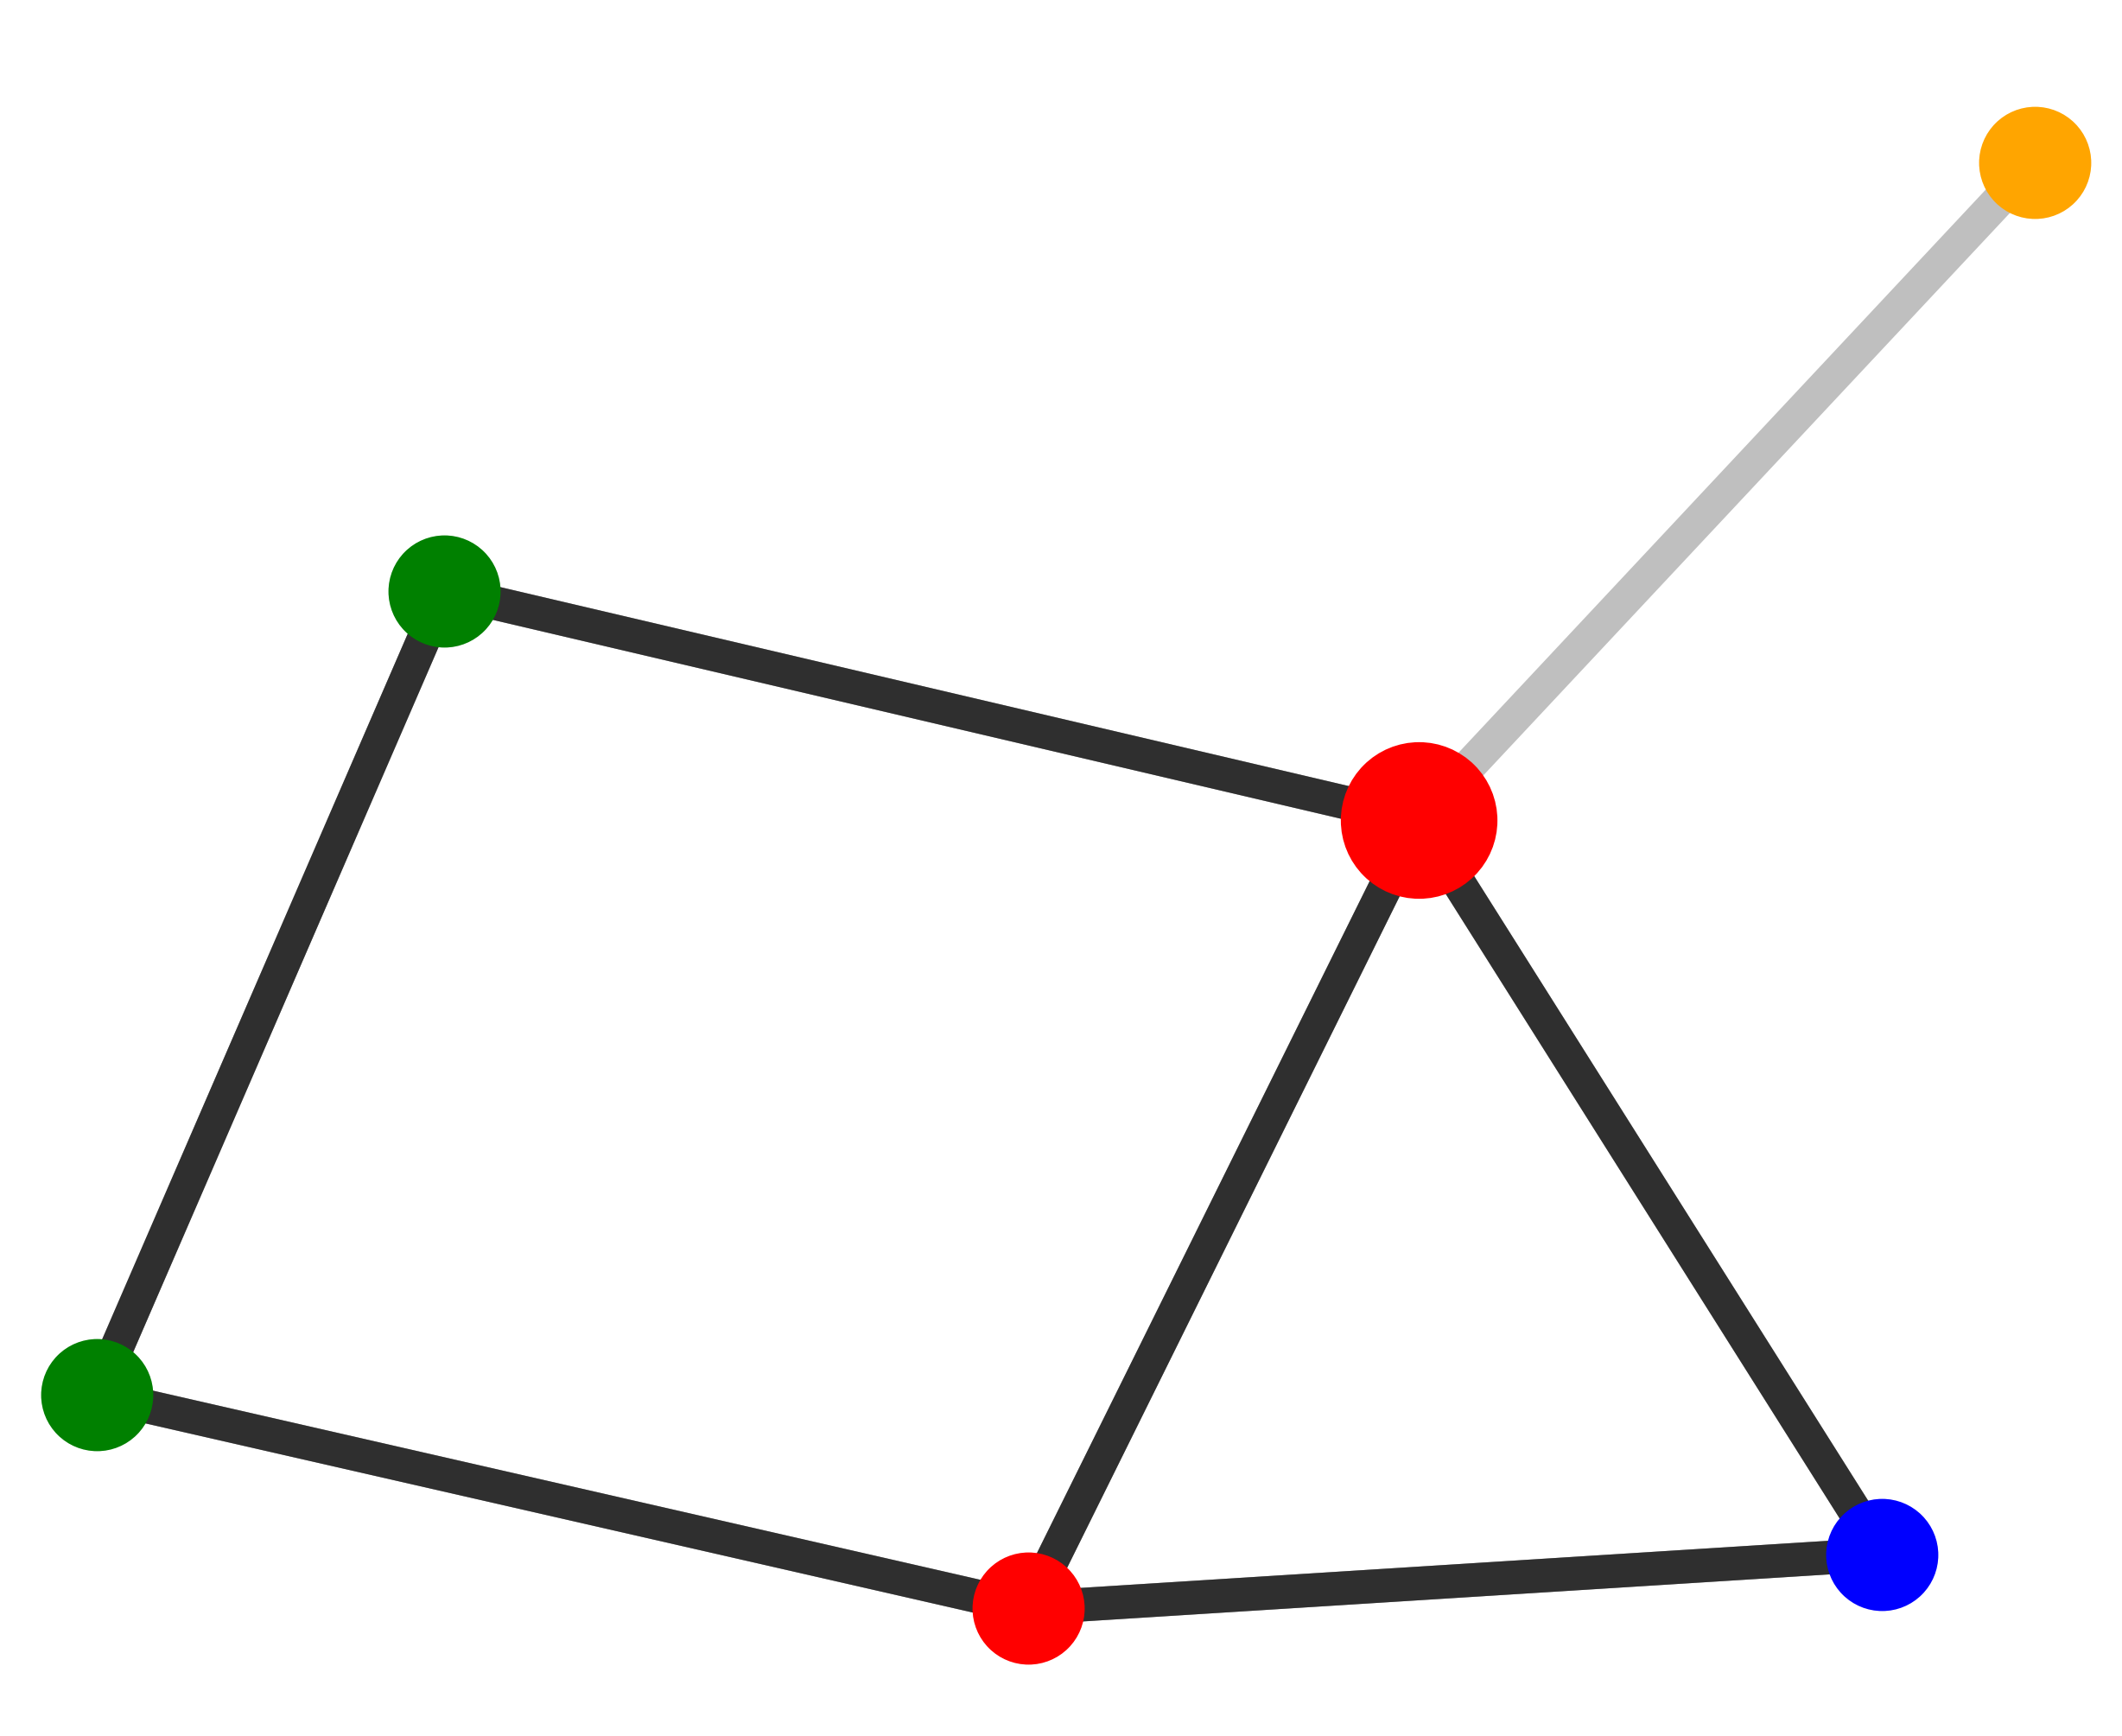
\includegraphics[width=.1\linewidth]{imgs/their_image-1.png}
% & 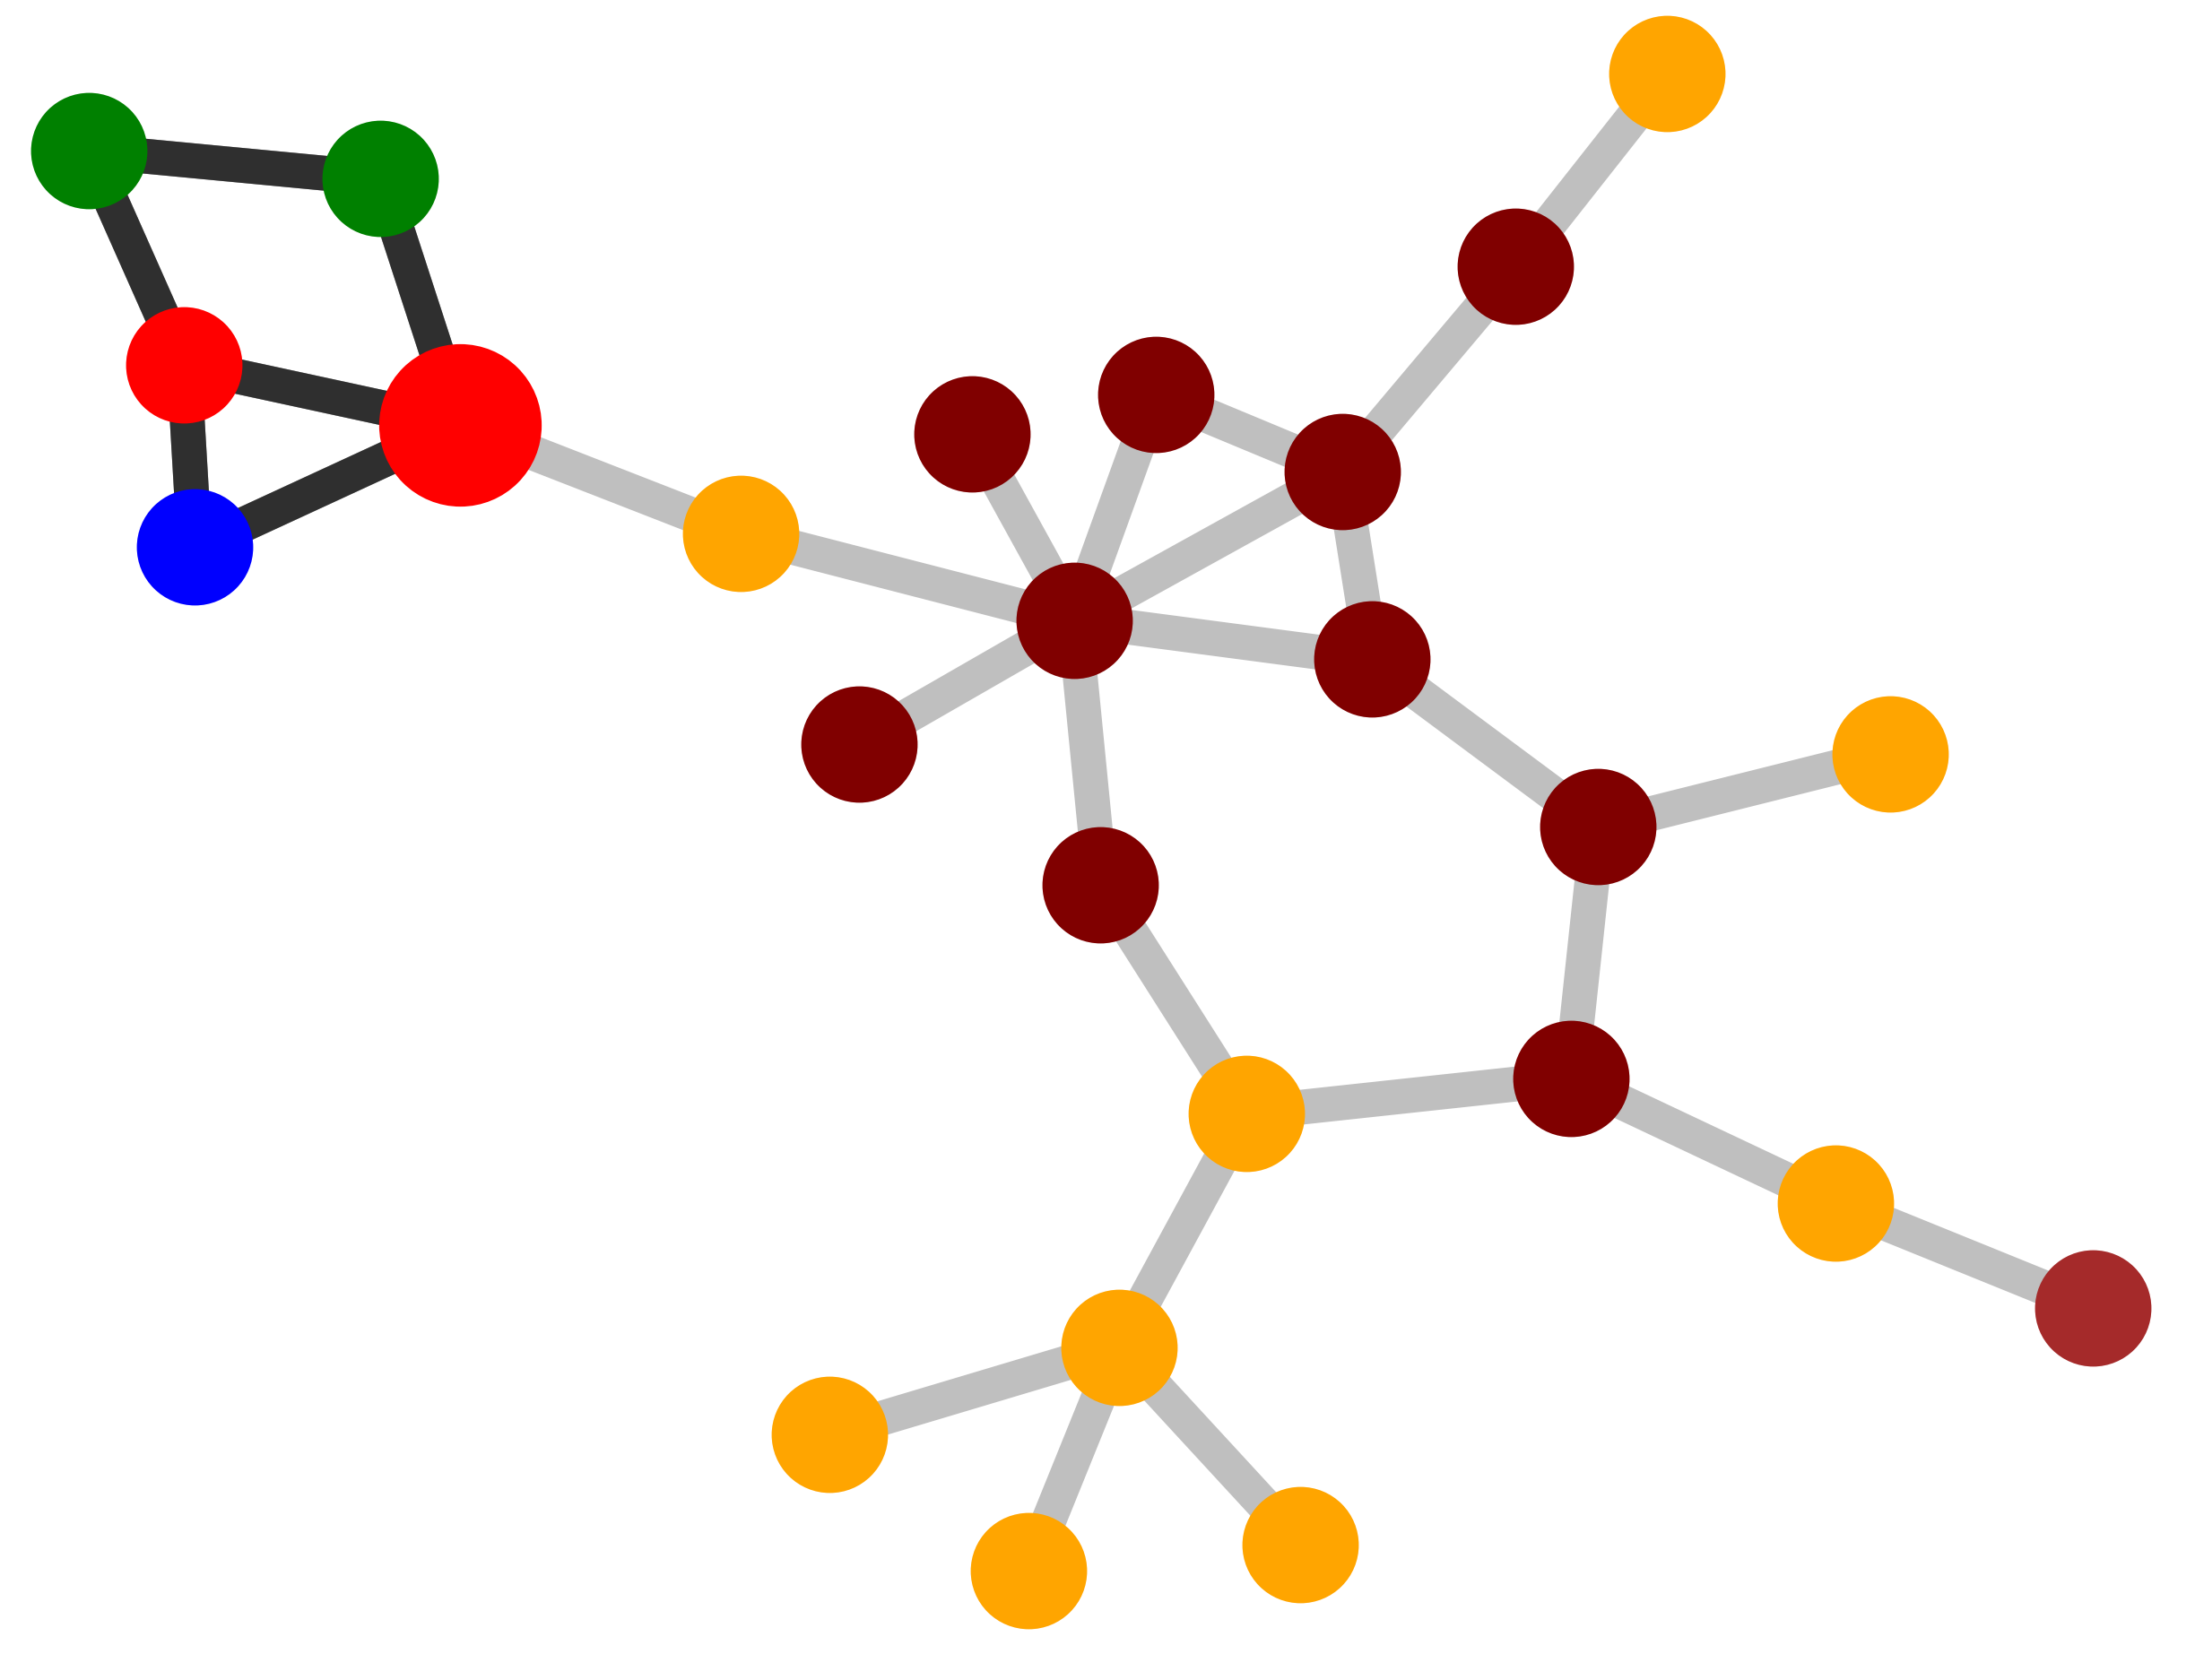
\includegraphics[width=.1\linewidth]{imgs/their_image-2.png} & 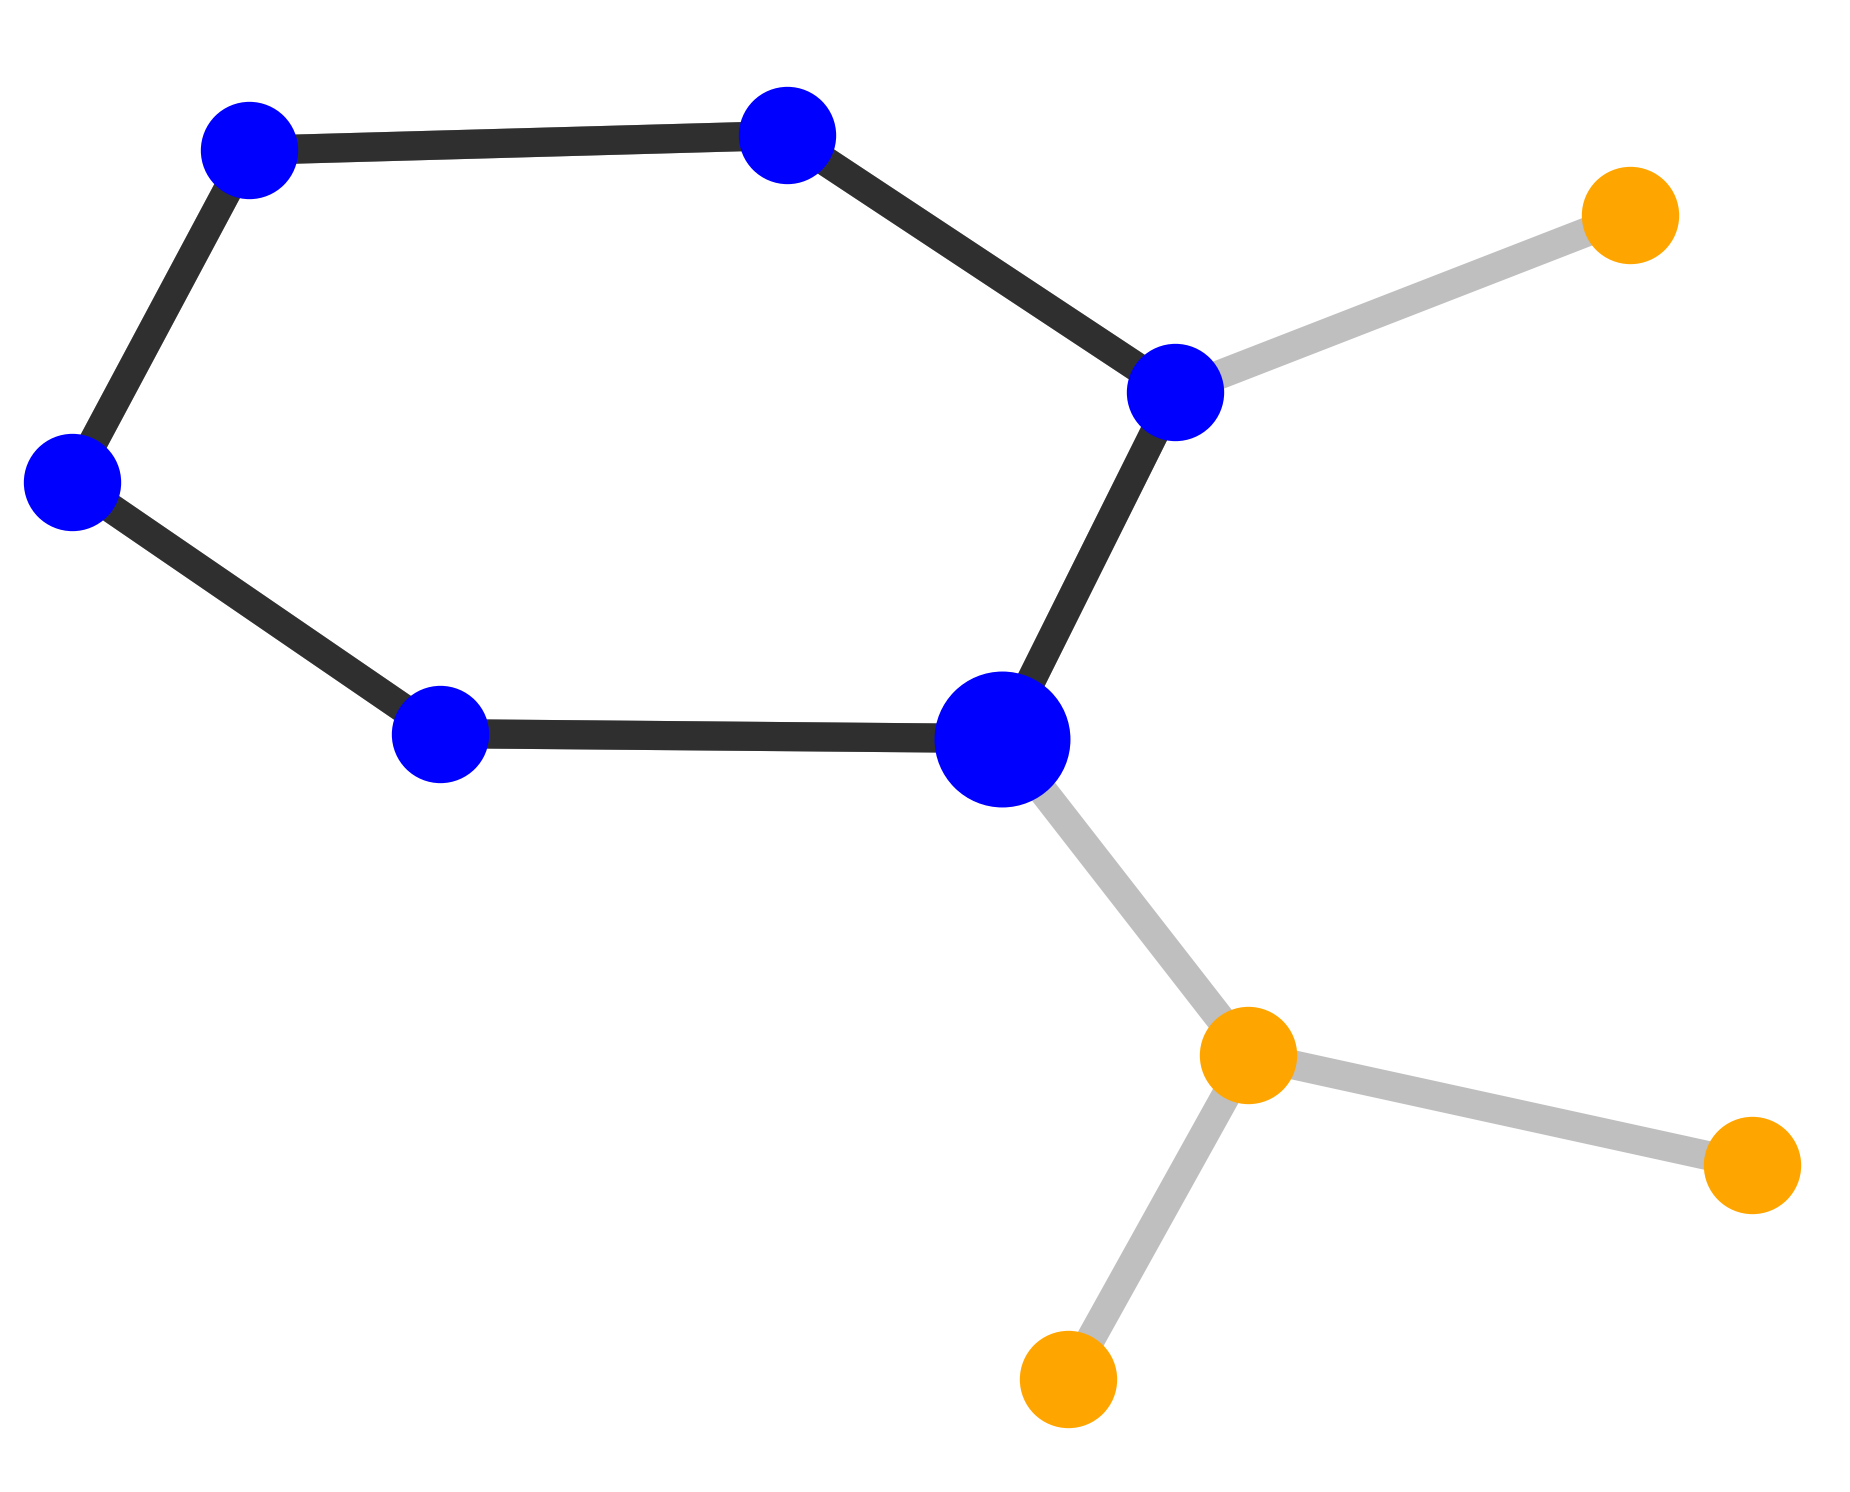
\includegraphics[width=.1\linewidth]{imgs/their_image-3.png} & \multicolumn{1}{l|}{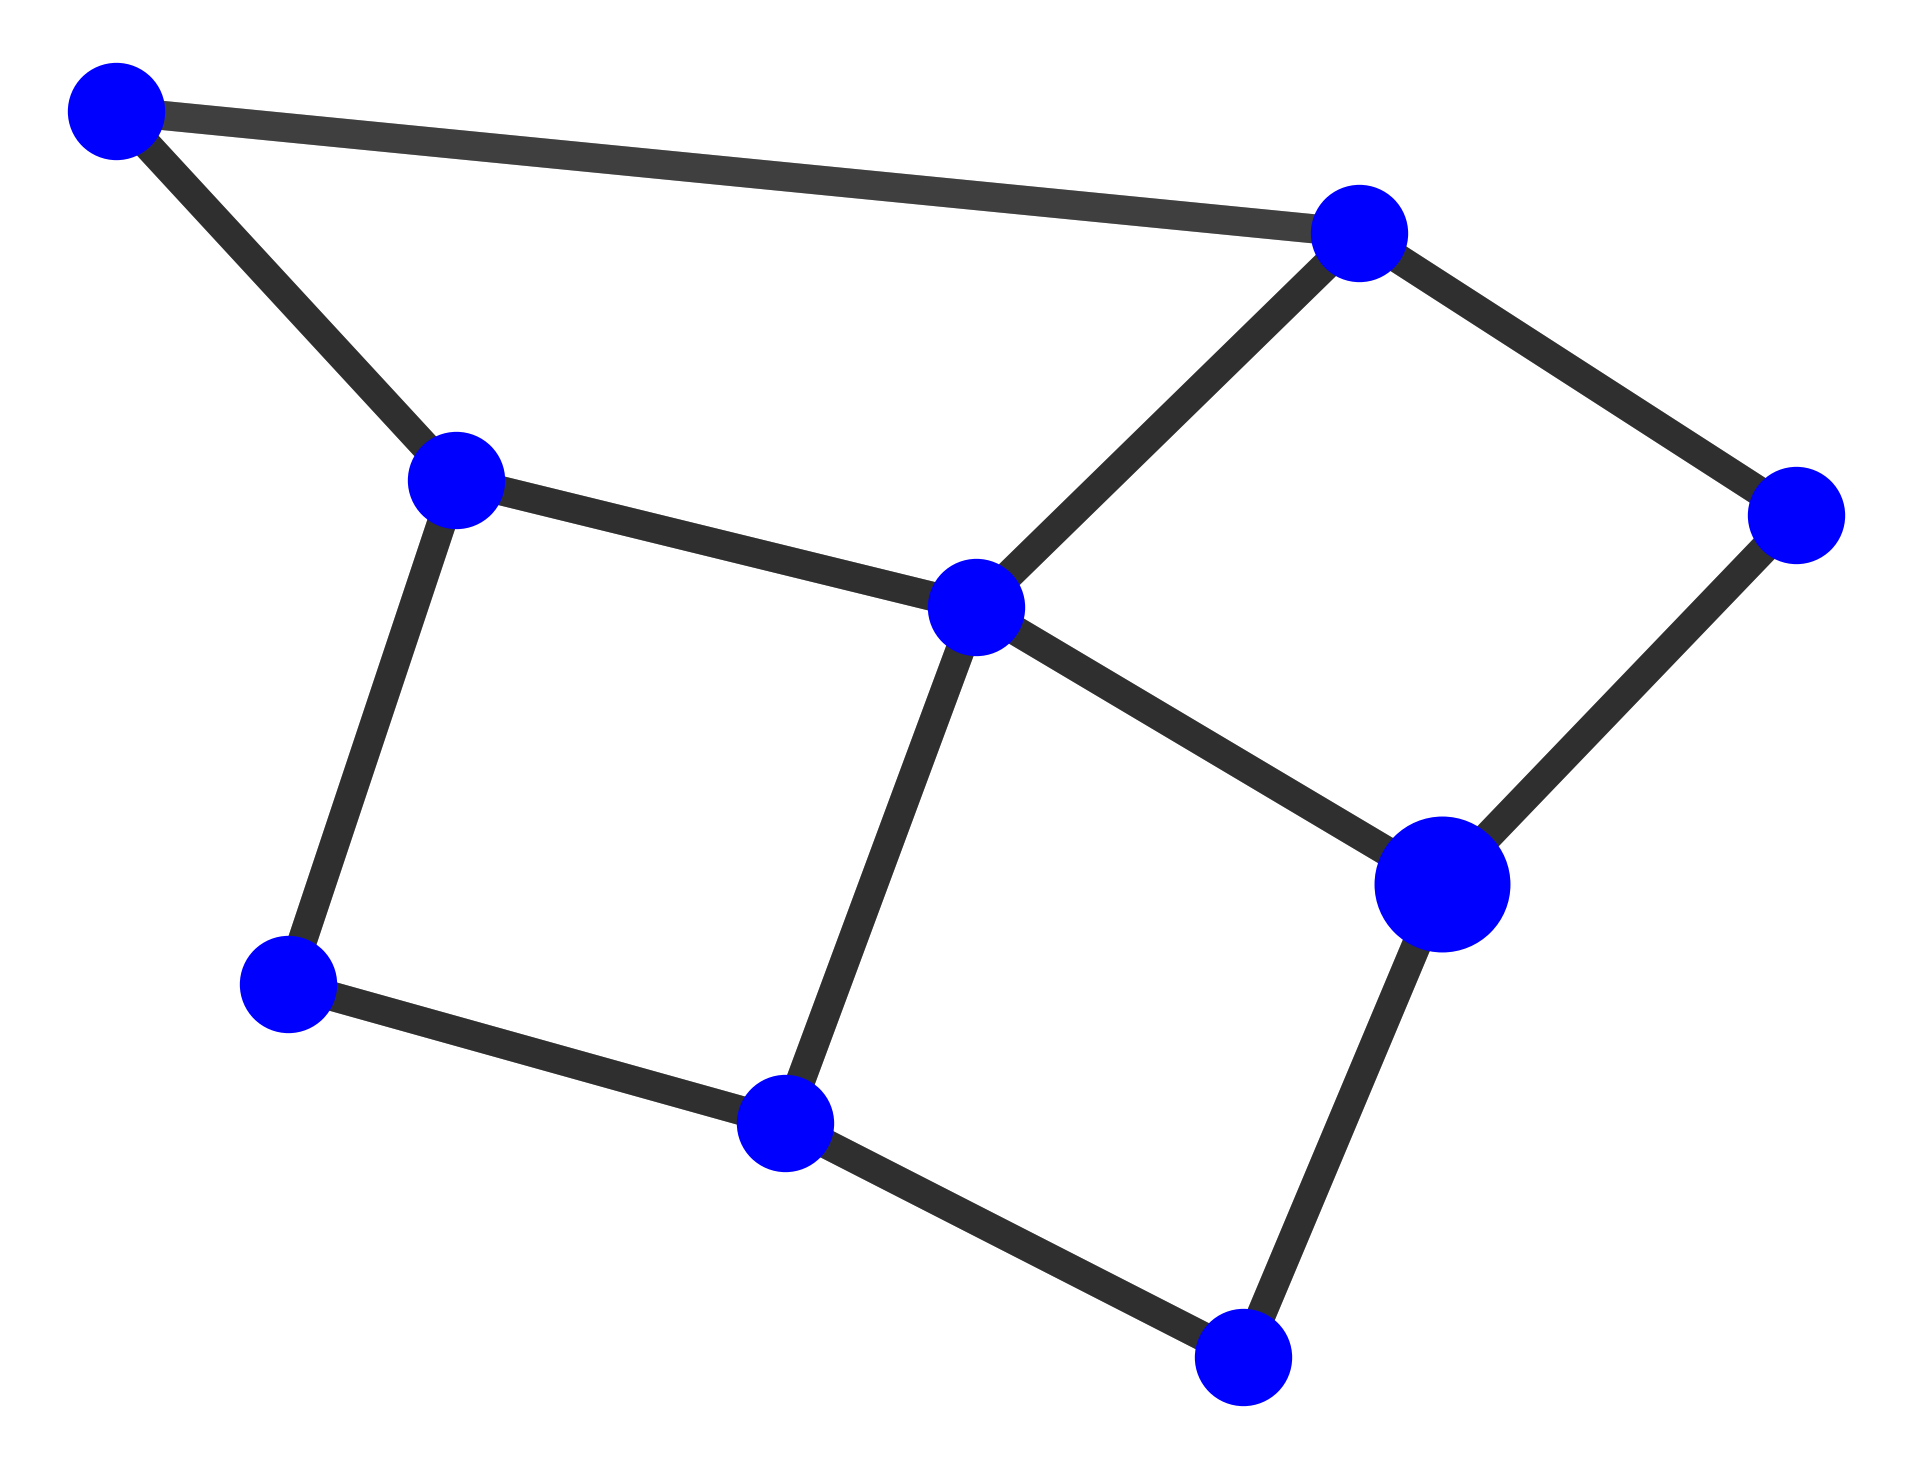
\includegraphics[width=.1\linewidth]{imgs/their_image-4.png}} & 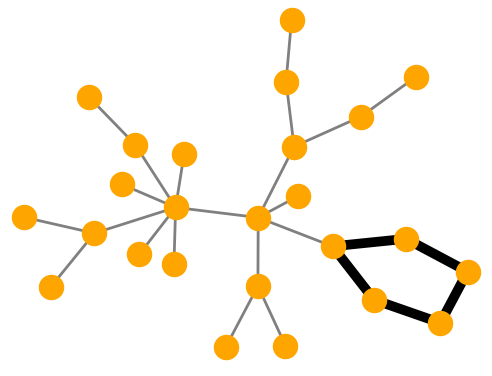
\includegraphics[width=.1\linewidth]{imgs/their_image-5.png} & 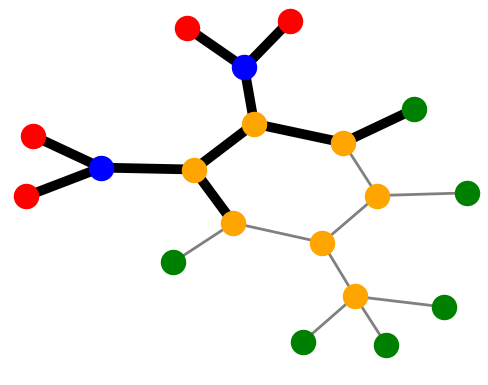
\includegraphics[width=.1\linewidth]{imgs/their_image-6.png} \\
% Reproduced & 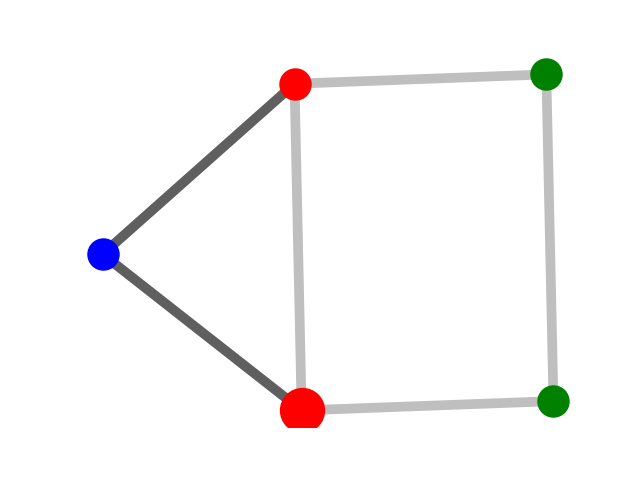
\includegraphics[width=.1\linewidth]{imgs/replication/syn1.png}
% & 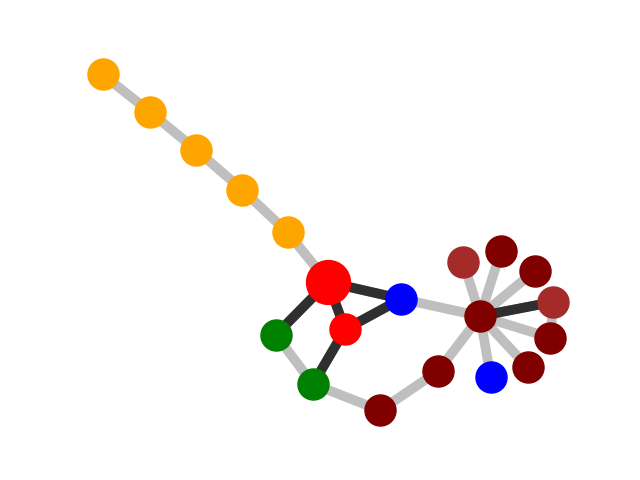
\includegraphics[width=.1\linewidth]{imgs/replication/syn2.png} & 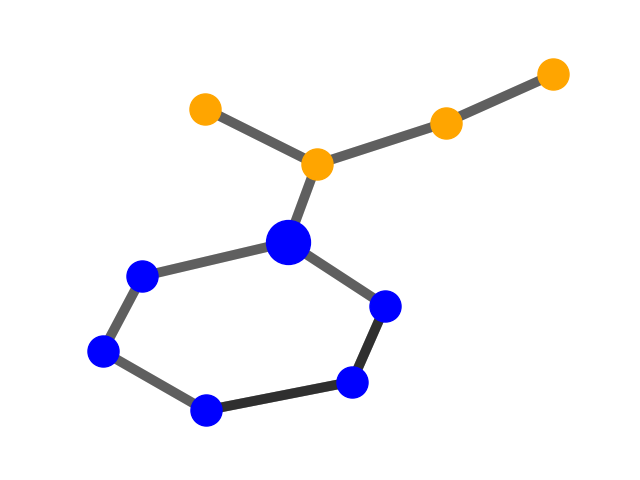
\includegraphics[width=.1\linewidth]{imgs/replication/syn3.png} & \multicolumn{1}{l|}{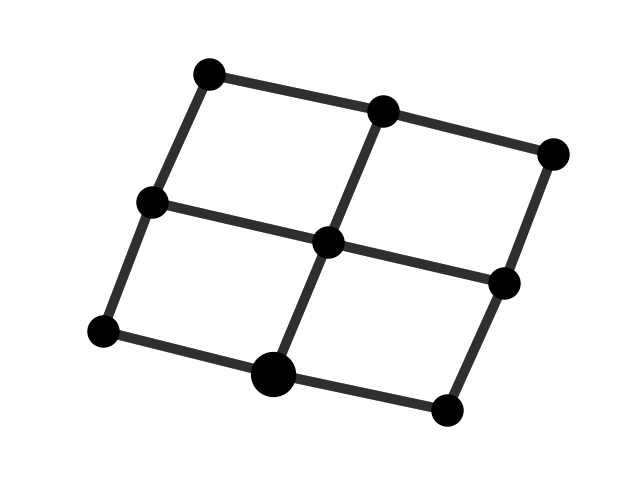
\includegraphics[width=.1\linewidth]{imgs/replication/syn4.png}} & img & 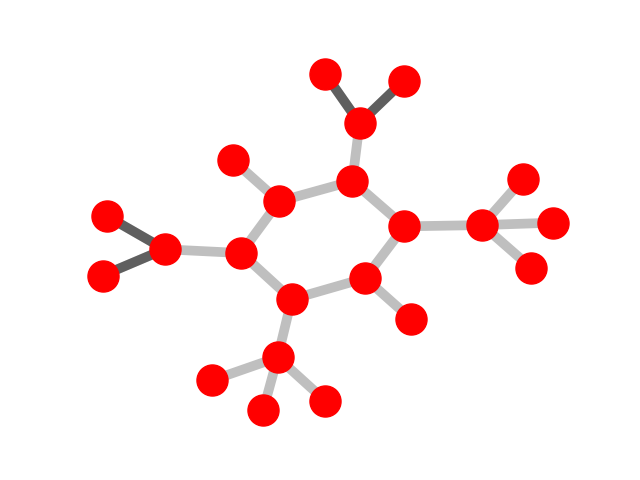
\includegraphics[width=.1\linewidth]{imgs/replication/85.png} \\ \hline
% \multicolumn{7}{l}{\textbf{Explanation AUC}} \\ \hline
% Original & 0.963 ± 0.011 & 0.945 ± 0.019 & 0.987 ± 0.007 & \multicolumn{1}{l|}{0.907 ± 0.014} & 0.926 ± 0.021 & 0.873 ± 0.013 \\ \hline
% Reproduced & 0.977 ± 0.006 & 0.970 ± 0.006 & 0.534 ± 0.186 & \multicolumn{1}{l|}{0.649 ± 0.045} & x.xx & 0.843 ± 0.084 \\ \hline
% \multicolumn{7}{l}{\textbf{Inference Time (ms)}} \\ \hline
% Reproduced & 3.56 & 5.29 & 0.40 & \multicolumn{1}{l|}{0.47} & x.xx & 2.09 \\ \bottomrule
% \end{tabular}
% \caption{Reproduction results}
% \label{tab:reproduction_results}
% \end{table}

% \paragraph{Qualitative}
% The replicated qualitative evaluation is very similar to the original results. PGExplainer is very capable of finding the motifs in the graphs and highlighting their edges. 

% \paragraph{Quantitative}
% The replicated quantitative evaluation shows results that are significantly different from the originals. Interestingly, the difference occurs in a different dataset then where the difference was observed in model accuracy. Despite the difference in validation and test accuracy between the replicated and the original model that is explained, the AUC score of the PGExplainer is very similar. On the other hand, the replicated evaluation of the tree-based graphs scores significantly lower, despite having very sensible qualitative explanations. One potential reason for this is the entropy and size regularization used in the PGExplainer. The configuration provided by the original codebase differ from the other datasets significantly for the tree-based datasets.

% \paragraph{Efficiency}
% Despite being evaluated using a considerably less powerful machine, and without utilizing a GPU, our implementation greatly outperforms the original implementation. 

% \subsection{Discussion}
% Based on the paper alone it is impossible to replicate the results presented in the paper, even if the complications of the evaluation itself are ignored. However, as the results presented above show, even with the provided codebase replicating the presented results is still not possible. First, the code base is badly structured and does not contain a central place describing the used configurations for training the models. Because of this a number of things remained unclear about the configuration of the models that might have lead to the reduced accuracy. For example, the training script configuration contained the possibility to use weight sharing and dropout to prevent over-fitting, but this is not used in any of the models. We hypothesize that this might be used for improving the accuracy of the BA-community model. 

% The replicated quantitative, qualitative and efficiency experiments similarly show that it is hard to reproduce the results prevented in the paper. Again, the main configuration files required to faithfully replicate the main results are missing. We believe that this effect is worsened by the crucial role of badly documented hyper parameters such as the entropy and size regularization coefficients. In the qualitative evaluation we expect that the importance of these hyper-parameters is hidden by the handpicked number of edges show in the explanation. The effect of these parameters will be further explored in the extended reproduction.



% Start with a high-level overview of your results. Does your work support the claims you listed in section 2.1? Keep this section as factual and precise as possible, reserve your judgement and discussion points for the next "Discussion" section. 

% Go into each individual result you have, say how it relates to one of the claims and explain what your result is. Logically group related results into sections. Clearly state if you have gone beyond the original paper to run additional experiments and how they relate to the original claims. 

% \subsection{Result 1}

% \subsection{Result 2}

% \subsection{Additional results not present in the original paper}

\section{Results} \label{sec:reproduction}

We first test whether the HGN \cite{hgn} can learn the dynamics of the four presented physical systems by measuring the average mean squared error (MSE) of the pixel reconstructions of each predicted frame.
Furthermore, we test the original HGN architecture along with different modifications: a version trained with Euler integration rather than Leapfrog integration (HGN Euler),
%a version trained with no transformer network (HGN no $f_\psi$),
and a version that does not include sampling from the posterior $q_\phi(\bm{z}|\bm{x}_0 ... \bm{x}_T)$ (HGN determ). Since we could not find suitable GECO\cite{geco} hyperparameters, we use a fixed Lagrange multiplier\cite{beta-vae} in all the experiments.
%To test HNN, we use the implementation provided by \cite{hnn} known as pixelHNN.
%Similarly to \cite{hgn}, we test HNN with a modification of the architecture to closely match the HGN (HNN Conv).

\begin{table}[]
    \centering
    \resizebox{\textwidth}{!}{%
    \begin{tabular}{c c c c c c c c c}
     \Xhline{3\arrayrulewidth}
     \textsc{Model} & \multicolumn{2}{c}{\textsc{Mass-spring}} & \multicolumn{2}{c}{\textsc{Pendulum}} & \multicolumn{2}{c}{\textsc{Two-body}} & \multicolumn{2}{c}{\textsc{Three-body}} \\
     & \textsc{Train} & \textsc{Test} & \textsc{Train} & \textsc{Test}& \textsc{Train} & \textsc{Test}& \textsc{Train} & \textsc{Test}\\
    \Xhline{3\arrayrulewidth}
     
    Orig. \textsc{HGN (Euler)} \cite{hgn} & $3.67 \pm 1.09$ & $6.2 \pm 2.69$ & $5.43 \pm 2.53$ & $10.93 \pm 4.32$ & $6.62 \pm 3.93$ & $15.06 \pm 7.01$ & $7.51 \pm 3.49$ & $9.4 \pm 3.92$ \\
    Orig. \textsc{HGN (Determ)} \cite{hgn} & $0.23 \pm 0.23$ & $3.07 \pm 1.06$ & $0.79 \pm 1.24$ & $10.68 \pm 3.19$ & $2.34 \pm 2.3$ & $14.47 \pm 5.24$ & $4.1 \pm 2.05$ & $5.17 \pm 1.96$ \\
    %Orig. \textsc{HGN (No $f_\psi$)} \cite{hgn} & $4.95 \pm 1.71$ & $7.04 \pm 2.55$ & $6.83 \pm 3.29$ & $13.98 \pm 4.94$ & $6.35 \pm 3.86$ & $16.49 \pm 6.6$ & $8.37 \pm 3.13$ & $10.41 \pm 3.72$ \\
    Orig. \textsc{HGN (Leapfrog)} \cite{hgn} & $3.84 \pm 1.07$ & $6.23 \pm 2.03$ & $4.9 \pm 1.86$ & $11.72 \pm 4.14$ & $6.36 \pm 3.29$ & $16.47 \pm 7.15$ & $7.88 \pm 3.55$ & $9.8 \pm 3.72$ \\
     \Xhline{3\arrayrulewidth}
     \textsc{HGN (Euler)} ours & $9.05 \pm 0.02$ & $9.06 \pm 0.05$ & $17.79 \pm 0.06$ & $17.86 \pm 0.13$ & $3.84 \pm 0.01$ & $3.85 \pm 0.02$ & $1.99 \pm 0.01$ & $1.99 \pm 0.01$ \\
     \textsc{HGN (Determ)} ours & $7.10 \pm 0.01$ & $7.10 \pm 0.03$ & $14.11 \pm 0.05$ & $14.14 \pm 0.12$ & $3.92 \pm 0.02$ & $3.93 \pm 0.02$ & $4.14 \pm 0.01$ & $4.13 \pm 0.02$ \\

     \textsc{HGN (Leapfrog)} ours & $7.11 \pm 0.01$ & $7.12 \pm 0.03$ & $14.89 \pm 0.05$ & $14.97 \pm 0.1$ & $3.36 \pm 0.01$ & $3.36 \pm 0.02$ & $8.81 \pm 0.01$ & $8.81 \pm 0.01$ \\
     \Xhline{3\arrayrulewidth}
     \textsc{HGN (Euler)} ours \textit{5-frame inference} & $42.09\pm 0.14$ & $41.98\pm 0.32$ & $47.06\pm 0.17$ & $47.03\pm 0.39$ & $6.46\pm 0.03$ & $6.52 \pm 0.06$ & $8.18 \pm 0.01$ & $8.17 \pm 0.01$ \\
     \textsc{HGN (Determ)} ours \textit{5-frame inference}& $13.00 \pm 0.05$ & $13.04 \pm 0.11$ & $45.06\pm 0.19$ & $44.89 \pm 0.42$ & $10.95\pm 0.02$ & $10.97 \pm 0.05$ & $3.72\pm 0.01$ & $3.72\pm 0.02$ \\
     \textsc{HGN (Leapfrog)} ours \textit{5-frame inference}& $12.15 \pm 0.05$ & $12.21 \pm 0.11$ & $44.29\pm 0.19$ & $44.12\pm 0.42$ & $6.28 \pm 0.03$ & $6.33 \pm 0.06$ & $3.35\pm 0.01$ & $3.35\pm 0.02$ \\
     \Xhline{3\arrayrulewidth}
    
    \end{tabular}}
    \vspace{0.25cm}
    \caption{Average pixel MSE of the reconstruction of a 30-frame rollout sequence on the test and train datasets of the four physical systems presented by \cite{hgn}. All the values are multiplied by $10^4$. We show our results (second and third group) along with the ones reported by the original authors (first group). In the second group, we train to reconstruct the whole inputted sequence (as an autoencoder) and in the third group, we train by inputting only the first 5 frames.}
    \label{tab:reproduction}
\end{table}

Table \ref{tab:reproduction} shows the results of the experiments described previously along with the results of the original authors. As it can be seen, we achieve average pixel reconstruction errors that are similar (30\% avg absolute error w.r.t. the reported values on the test set using Leapfrog integrator) to the ones reported in the original paper when reconstructing the same sequence that is inputted (we call this version \textit{autoencode}).
However, when attempting to train to reconstruct a rollout given only the first 5 frames our model performs poorly, with 107\% average absolute error on the test set, using Leapfrog integrator.
% This might be for several reasons that will be discussed in Sec. \ref{sec:disc}.
%In general, we can observe that our HGN and the proposed modifications learned well on the four physical systems.
% As it can be observed, the results reported by both versions of the HNN are one order of magnitude higher than the four versions of the HGN. Visual inspections of the results provided by HNN show that the network simply learned to output a static image.

\begin{figure}
    \centering
    \begin{subfigure}{.48\textwidth}
        \centering
        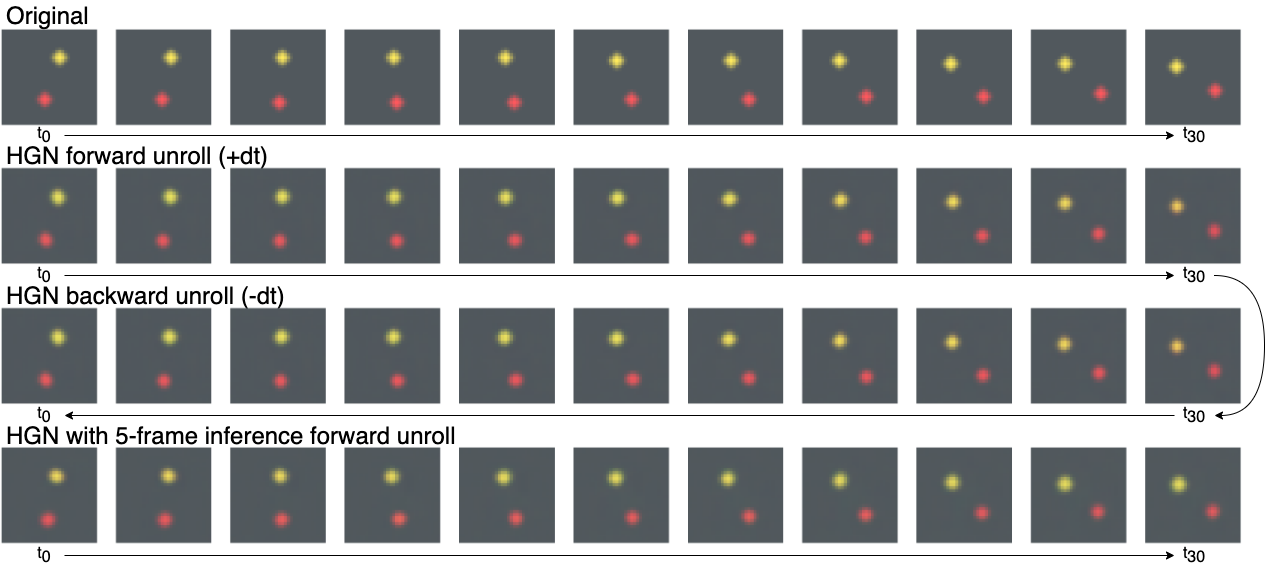
\includegraphics[width=.9\linewidth]{../openreview/pictures/rollout_samples/new_forward_unroll_2_body.png}
        \label{fig:rollout-3-body}
        \caption{}
    \end{subfigure}
    \begin{subfigure}{.48\textwidth}
        \centering
        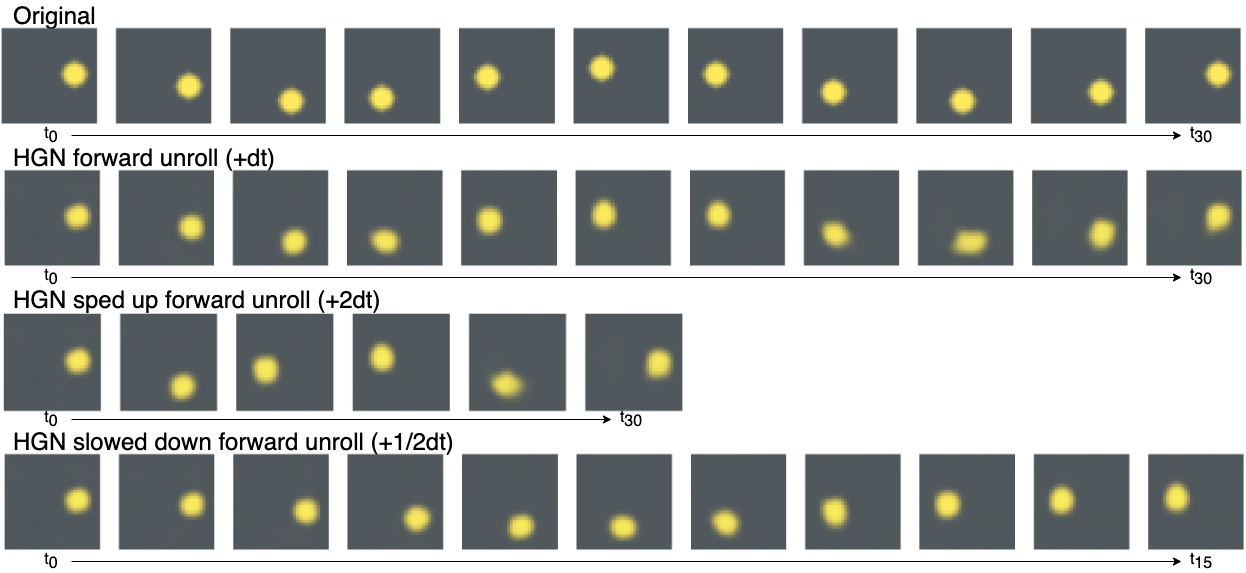
\includegraphics[width=.9\linewidth]{../openreview/pictures/rollout_samples/new_forward_backward_unroll_pendulum.png}
        \caption{}
        \label{fig:rollout-pendulum}
    \end{subfigure}
    \caption{(a) Reconstruction of a sequence of the 2-body system along with a backward unroll of the data from the final state, and a forward rollout of the HGN trained using state inference from the first 5 frames. (b) Reconstruction of a sequence of the pendulum system along with a sped up and a slowed down forward rollout.}
    \label{fig:rollout_back_forth}
\end{figure}

In Figure \ref{fig:rollout_back_forth}, we show some qualitative examples of the reconstructions obtained by the full version of HGN. The model can reconstruct the samples and its rollouts can be reversed in time, sped up, or slowed down by changing the value of the time step used in the integrator. Since the HGN is designed as a generative model, we can sample from the latent space to produce initial conditions and perform their time evolution. We show some rollouts obtained this way in figure \ref{fig:samples}. We observe that our model is only able to generate plausible and diverse samples in the mass-spring dataset.
This behavior is different than the one shown by \cite{hgn} and might be caused by different hyper-parameter configurations in the training procedure or some implementation mistake.
% Later discussion with the authors revealed that they did not input the whole rollout to the encoder but just the first five frames, which was not explained in the paper. Since we received the information too late, we could not run all the experiments again.
% However, we tried this modification in the \textit{mass-spring} dataset, achieving a reconstruction loss of $1.4\times 10^{-3}$, which is very similar to authors results. 


% - The way we assess error: larger bodies with more movement gets more penalized
% - 2-3 bodies move slower and seems better for our model
% - Seems that our hyper-parameter choice is better at physics and theirs better at reconstruction
% - Identify good/bad physiscs and good/bad reconstructions


% Below we comment on the results reported for each environment.

% We takl about mass spring. then talk about pendulum. 
We achieve slightly larger MSE in the autoencode version and significantly larger in the 5-frame inference problem on both the mass-spring and pendulum.
The latter presents roughly double MSE probably because of a wider span of movement.
In general, these two environments show worse results in comparison to two/three-bodies.
For these last cases, our implementation using the \textit{autoencode} setting outperforms the original HGN \cite{hgn}, and when using the \textit{5-frame inference} the results are similar.
As we can see, these two environments show much less average pixel MSE compared to the first ones (almost one order of magnitude).
We believe this may be due to the differences when rendering the instances of each dataset.
The elements appearing in mass-spring and pendulum (represented by a large yellow ball) are larger than the ones present in the two/three bodies (two/three small coloured balls).
Because of this, it would be reasonable to assume that localization errors are more penalized in the first two environments, since the total difference in areas is larger.
Furthermore, the dynamics representing mass-spring and pendulum show faster movements in comparison to two/three-bodies, resulting in being harder to represent with our HGN.
Consequently, we hypothesise the following: larger elements and faster dynamics, produces higher average MSE on our model regardless of the difficulty of the environment physics.
However, this is not the case for the original author's results, who seem to struggle more on the two/three-bodies.
Surprisingly, it seems that our hyperparameter and architecture choices led to poorer reconstruction capabilities (higher MSE) but learning better physics (qualitatively more realistic movements).
% The error gets severely exacerbated when only inputting the first 5 frames of the sequence.

% In fact, 2 bodies are tal tal ,3 bodies are tal tal, and it is because of the previous assumption.






% \begin{itemize}
%     \item \textbf{Mass-spring and Pendulum:}

    
%     In comparison, both environments seem to be harder for us to learn than the multiple bodies ones.
     
%     % Surprisingly, it seems that our hyperparameter and architecture choices let to learning better physics but poorer reconstruction capabilities.

%     \item \textbf{Two-body and Three-body:} As we observe, our implementation using the \textit{autoencode} setting is able to outperform the original HGN \cite{hgn}. On the other hand, when using \textit{5-frame inference}, the results are still comparable. 
    
%     %Although it is hard to draw an exact conclusion on the factors causing these results, we can see the instances represented in the \textit{two/three-body} dataset are smaller compared to the ones in the \textit{mass-spring} or \textit{pendulum} (see Figure \ref{fig:datasets} for reference). Moreover, the dynamics of the \textit{two/three-body} systems are steadier. These two factors
    
%     Autoencode is better than them, 5-frames is similar
%     \item \textbf{Three-body:} Both autoencode and 5-frame better than them. Why?
% \end{itemize}


\begin{figure}
    \centering
    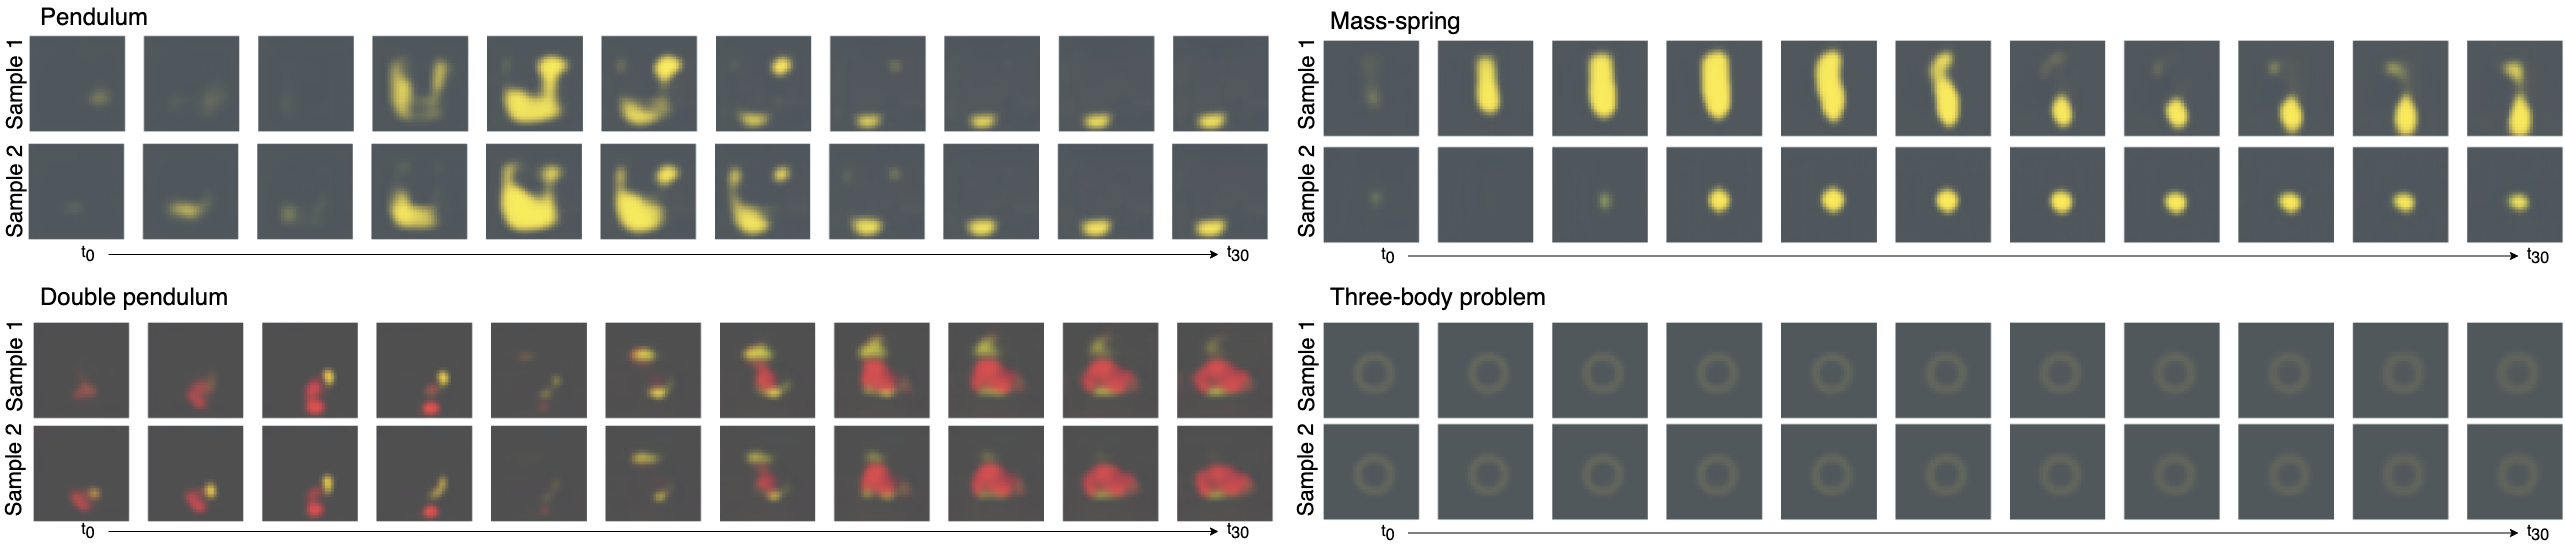
\includegraphics[width=\textwidth]{../openreview/pictures/rollout_samples/new_sampling.png}
    \caption{Examples of sample rollouts from the latent space for different physical systems.}
    \label{fig:samples}
\end{figure}

\subsection{Additional experiments} \label{sec:additional_experiments}

\paragraph{GECO parameter search} \label{sec:hyperparam_search} The paper does not provide the values of GECO \cite{geco} used. In GECO, the Lagrangian multiplier is optimized at each step with a rate $\gamma$.
Figure \ref{fig:geco_search} shows the behavior of GECO for $\gamma \in \{0.1, 0.05, 0.01\}$ in terms of reconstruction loss and KL divergence. Higher values of $\beta$ give a better reconstruction loss but greatly increase the KL divergence. %In our experiments we generally use $\beta = 0.05$, which provides a good trade-off, or $\beta = 0.1$ for environments in which reconstruction is harder (e.g. pendulum).
However, we found that hyperparameters were not consistent among different environments and integrators. For this reason, we do not use GECO in our experiments.
\begin{figure}[]
\minipage{0.5\textwidth}
\centering
  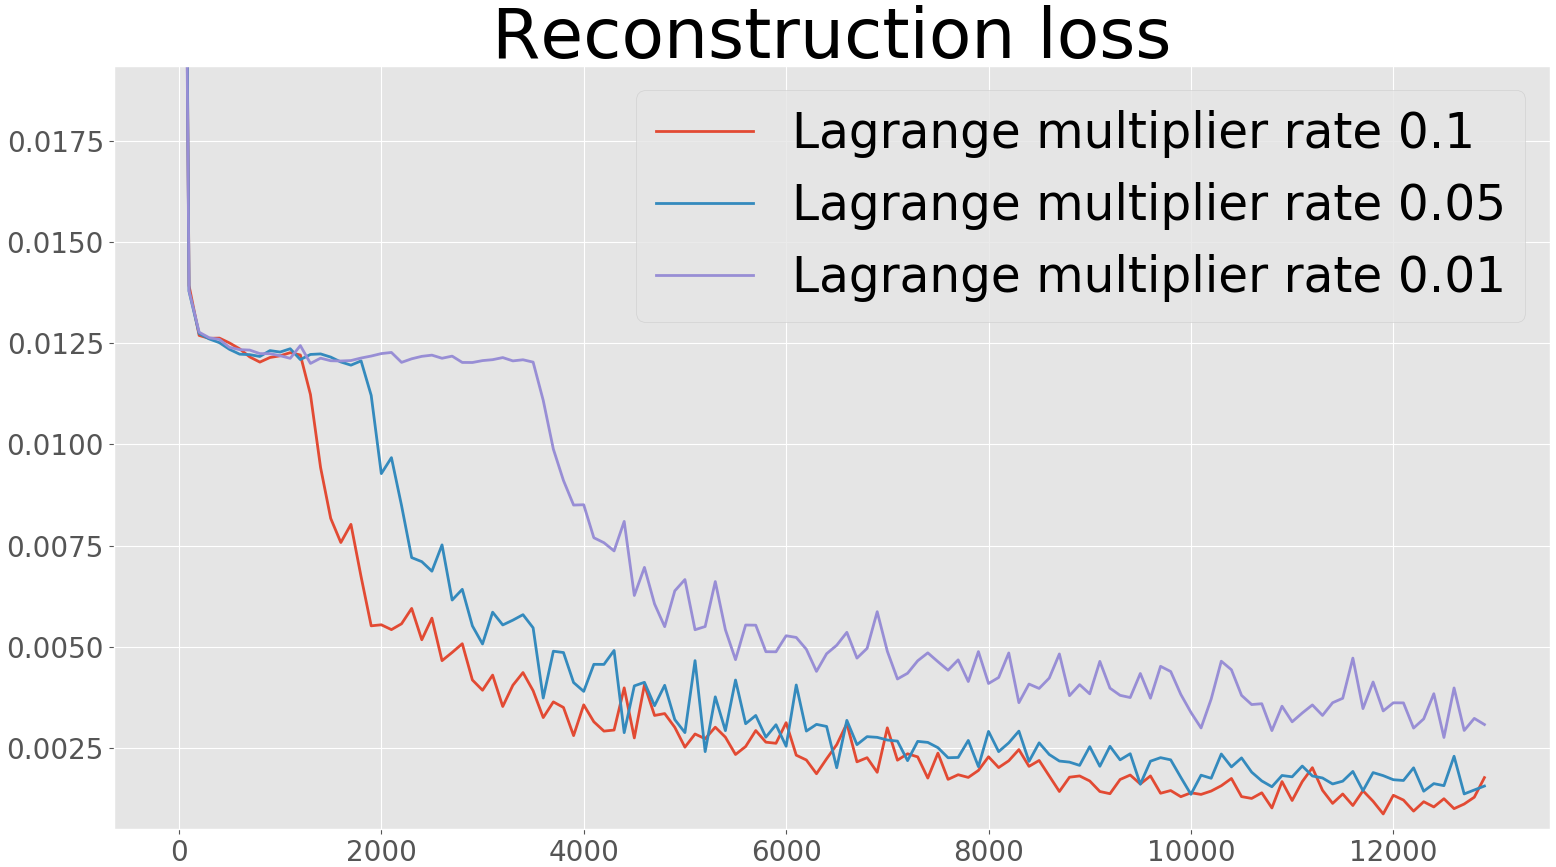
\includegraphics[width=0.8\linewidth]{../openreview/pictures/parameter_comparisons/lagrange_multiplier_comparison_rec_loss.png}
\endminipage\hfill
\minipage{0.5\textwidth}
\centering
  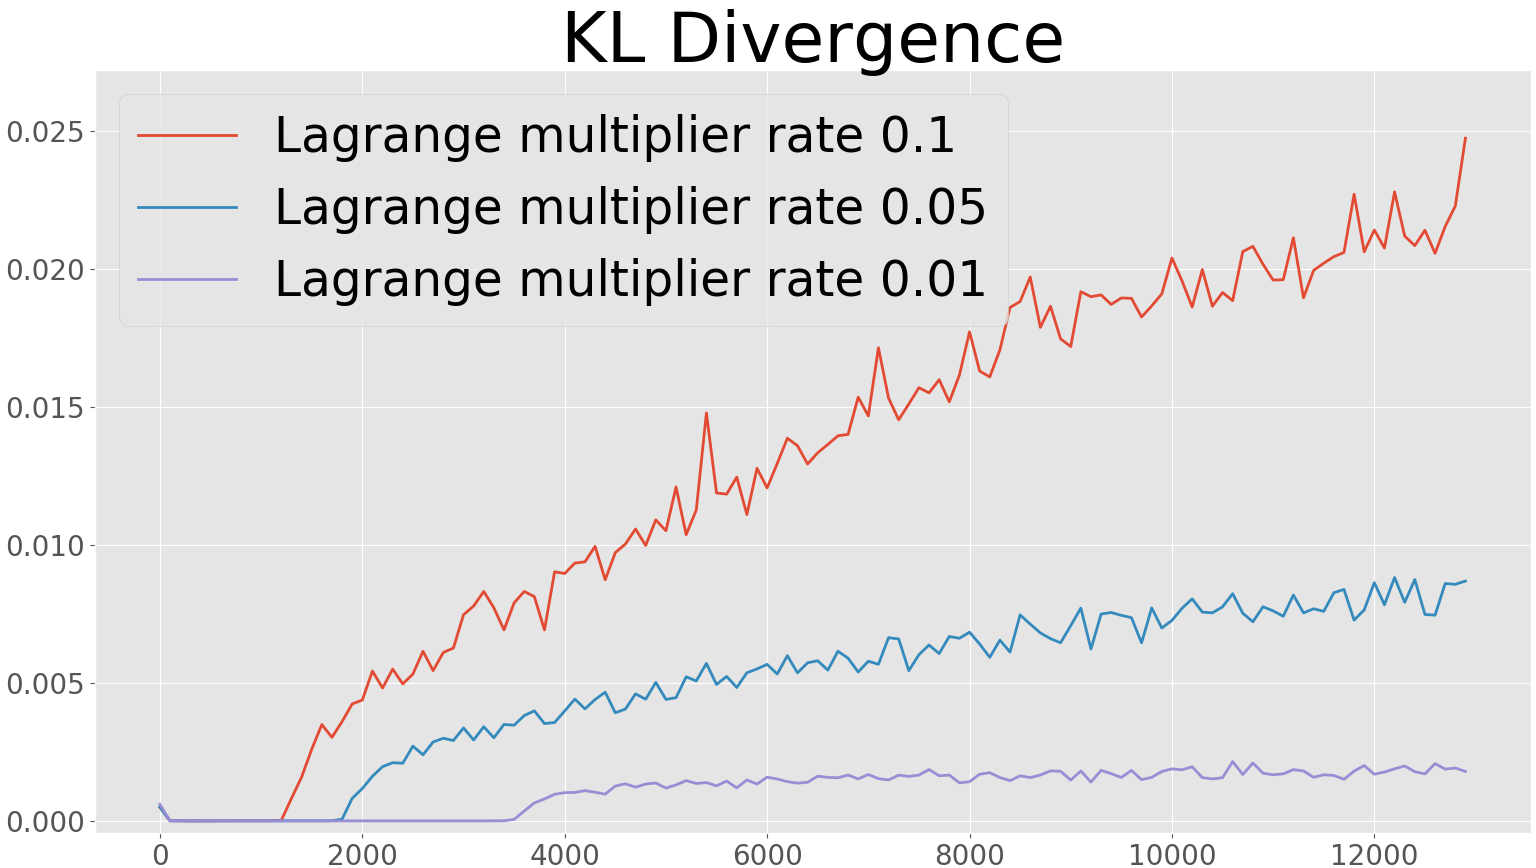
\includegraphics[width=0.8\linewidth]{../openreview/pictures/parameter_comparisons/lagrange_multiplier_comparison_kld.png}
\endminipage
\caption{Reconstruction loss and KL divergence for different GECO parameters in the Pendulum environment.}
\label{fig:geco_search}
\end{figure}


\paragraph{Integrators} \label{sec:integrators}
Performing the integration step is key to generate the time evolution of a rollout given the initial state. 
In the HGN paper \cite{hgn} the system is tested using Euler and Leapfrog integration. We wonder if using higher order integration methods might boost the performance of the rollout generation process.
% The Runge-Kutta integration is only used when training the HNN architecture \cite{hnn}. 
%We observed that one main disadvantage of Euler integration is that its errors accumulate rapidly over longer time periods.
Therefore, we implement and test the HGN architecture with two additional numerical integration methods: the Runge-Kutta's 4th-order integrator \cite{rk4} and the 4th-order Leapfrog integrator (Yoshida's algorithm \cite{yoshida1992symplectic}). Table \ref{tab:integrators} shows a comparison of all four integrators on the Pendulum dataset.
%For this reason other methods that involve more integration steps, such as the fourth-order Runge-Kutta integration (RK4) or the fourth-order Leapfrog (Yoshida's algorithm) \cite{yoshida1992symplectic} have been implemented.
Both Leapfrog and Yoshida are \textit{symplectic} integrators: they guarantee to preserve the special form of the Hamiltonian over time \cite{neal2011mcmc}.
% , at the cost of slower execution.

\begin{table}[]
    \centering

    \begin{tabular}{c c c c c}
     \Xhline{3\arrayrulewidth}
      & \textsc{Euler} & \textsc{Runge-kuta 4} & \textsc{Leapfrog} & \textsc{Yoshida}\\

     \Xhline{3\arrayrulewidth}
     pixel MSE & $17.86 \pm 0.13$ & $76.88 \pm 0.08$ & $14.97\pm 0.10$ & $14.70\pm 0.10$ \\
     $\mathcal{H}$ std & $3.81$ & $0$ & $1961.93$ & $1893.05$\\
     reconstr. time (s) & $0.32$ & $1.89$ & $0.96$ & $1.61$ \\

     \Xhline{3\arrayrulewidth}
    
    \end{tabular}
    \vspace{0.25cm}
    \caption{Comparison between four different integrators used to perform the time evolution in the HGN. The results are measured on the simple pendulum test set. The pixel MSE values have been multiplied by $10^4$.}
    \label{tab:integrators}
\end{table}

Table \ref{tab:integrators} shows the average pixel MSE, the averaged standard deviation of the output of the Hamiltonian network during testing, and the reconstruction time of a single batch ($\texttt{batch}=16$) using the different integration methods that we have described previously. The model has been trained on the simple pendulum dataset. As we can see, the reconstruction time increases when using higher-order integration methods, since they require more integration steps. In general, we see that Euler integration offers a fast and sufficiently reliable reconstruction of the rollouts. Moreover, we observe that the fourth-order symplectic integrator (Yoshida) achieves the best performance. Surprisingly, the symplectic integration methods show more variance in the output of the Hamiltonian networks throughout a single rollout. This behavior is unexpected since using a symplectic integration method should ideally keep the value of the Hamiltonian invariant. We conclude that more experiments need to be performed to guarantee that the implementation of both Leapfrog and Yoshida integration methods are faithful to their formulation.


\paragraph{Integrator modelling} We train the modified architecture of Section \ref{sec:integrator_modelling} on the Pendulum dataset for 5 epochs. The architecture is the same as HGN, but the Hamiltonian Network now outputs $\Delta q$ and $\Delta p$. The average MSE error over the whole Pendulum dataset is $1.485\times 10^{-3}$, while in the test set it is $1.493 \times 10^{-3}$, which are both very close ($\sim \pm 2\%$) to those of autoencoding HGN (see Table \ref{tab:reproduction}). The modified architecture is still capable of performing forward slow-motion rollouts by modifying $\Delta t$. We set $\Delta t' = \frac{\Delta t}{2}$ and we compute the average MSE of the slow-motion reconstruction over 100 rollouts. The modified architecture achieved an error of $8$x$10^{-4}$, while the standard HGN achieved $9$x$10^{-4}$. Note that reconstruction losses are smaller for slow-motion as the images change less between timesteps.



\paragraph{Extra environments}
Apart from the four physical systems presented by \cite{hgn} we test our re-implementation of the HGN with physical systems that do not have a simple Hamiltonian expression. As described previously, these are the damped harmonic oscillator and the double pendulum. On one hand, we are interested in a damped system since it introduces a dissipative term to the equations of motion; a feature that differs from the previous systems. On the other hand, the double pendulum is modelled by a non separable Hamiltonian: $\mathcal{H}(\textbf{q},\textbf{p}) \neq K(\textbf{p}) + V(\textbf{q})$ as described previously. In figure \ref{fig:extra} we show some visual examples of the reconstructions provided by the HGN trained on the two systems. As we can see, HGN is able to reconstruct the damped oscillator with high reliability. Regarding the double pendulum, we observe that the model reconstructs well small oscillations, but fails when the trajectory is too chaotic as expected. The average pixel MSE of the reconstructions of the damped oscillator and the double pendulum are $6.39\cdot 10^{-4}$ and $6.91\cdot 10^{-4}$ respectively. The HGN is able to provide better reconstructions for these systems in comparison to the mass-spring and pendulum systems.

\begin{figure}
    \centering
        \begin{subfigure}{.48\textwidth}
        \centering
        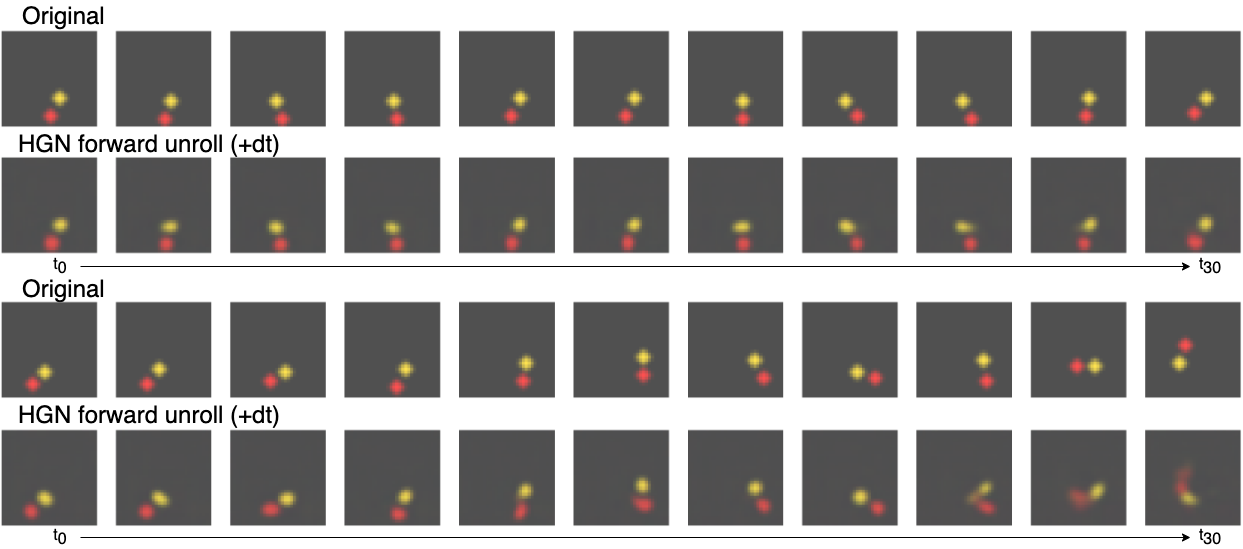
\includegraphics[width=\linewidth]{../openreview/pictures/rollout_samples/new_chaotic_pendulum_rollouts.png}
        \label{fig:a}
    \end{subfigure}
    \begin{subfigure}{.48\textwidth}
        \centering
        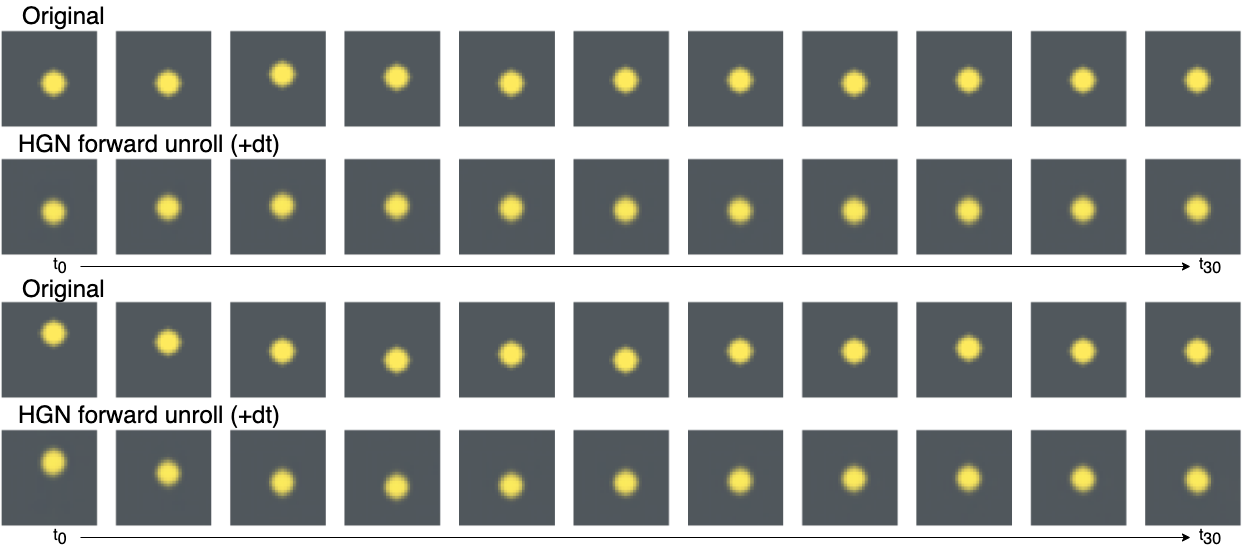
\includegraphics[width=\linewidth]{../openreview/pictures/rollout_samples/new_damped_spring_sample_rollout.png}
        \label{fig:b}
    \end{subfigure}
    \caption{Examples of reconstructions of the double pendulum (left) and the damped harmonic oscillator (right).}
    \label{fig:extra}
\end{figure}


\section{Discussion}

Evaluated on image classification, the central claims of \citet{rigl} hold true---\textit{RigL} outperforms existing sparse-to-sparse training methods and can also surpass other dense-to-sparse training methods with extended training. \textit{RigL} is fairly robust to its choice of hyperparameters, as they can be set independent of sparsity or initialization. We find that the choice of initialization has a greater impact on the final performance and compute requirement than the method itself. Considering the performance boost obtained by redistribution, proposing distributions that attain maximum performance given a FLOP budget could be an interesting future direction.\\

For computational reasons, our scope is restricted to small datasets such as CIFAR-10/100. \textit{RigL}'s applicability outside image classification---in Computer Vision and beyond (machine translation etc.) is not covered here.

\subsubsection{What was easy}
The authors' code covered most of the experiments in their paper and helped us validate the correctness of our replicated codebase. Additionally, the original paper is quite complete, straightforward to follow, and lacked any major errors.

\subsubsection{What was difficult}

Implementation details such as whether momentum buffers were accumulated sparsely or densely had a substantial impact on the performance of SNFS. Finding the right $\epsilon$ for ERK initialization required handling of edge cases---when a layer's capacity is exceeded. Hyperparameter tuning $(\alpha, \Delta T)$ involved multiple seeds and was compute-intensive.

\subsubsection{Communication with original authors}

We acknowledge and thank the original authors for their responsive communication, which helped clarify a great deal of implementation and evaluation specifics. Particularly, FLOP counting for various methods while taking into account the changing sparsity distribution. We also discussed experiments extending the original paper---as to whether the authors had carried out a similar study before.


\bibliographystyle{plain}
\small
\bibliography{reflist}

\end{document}
